\documentclass[a4paper]{article}
\usepackage[utf8]{inputenc}
\usepackage{hyperref}
\hypersetup{
	colorlinks,
	citecolor=black,
	filecolor=black,
	linkcolor=black,
	urlcolor=black
}
\usepackage{graphicx}
\usepackage{amssymb}
\usepackage{amsfonts}
\usepackage{amsmath}
\usepackage{pgfplots}
\usepackage{tikz}
\usepackage{tkz-euclide}
\usepgfplotslibrary{polar}
\usepgfplotslibrary{fillbetween}
\usetikzlibrary{pgfplots.polar}
\pgfplotsset{compat=1.18, width=\textwidth}
\usepackage{mathtools}
\usepackage[thinc]{esdiff}
\def\pgfplots@stacked@diff{}
\setlength\parindent{12pt}
\usepackage{tabularx}
\usepackage{makecell}
\usepackage{amsthm}
\usepackage{tabularx}
\usepackage[noEnd=true]{algpseudocodex}
\usepackage[a4paper, marginparwidth=80pt, top=5cm, bottom=5cm, left=3cm, right=5cm]{geometry}
\usepackage{marginnote}
\usepackage{polynom}
\usepackage{xfrac}
\usepackage{gensymb}
\usepackage{fancyhdr}
\usepackage{undertilde}
\usepackage{nicematrix}
\usepackage{float}

\DeclareMathOperator\cis{cis}
\DeclareMathOperator\Arg{Arg}

\pgfplotsset{polar default/.append style={xticklabels={,,
			$\frac{\pi}{6}$, $\frac{\pi}{3}$, $\frac{\pi}{2}$, $\frac{2\pi}{3}$,
			$\frac{5\pi}{6}$, $\pi$, $\frac{7\pi}{6}$, $\frac{4\pi}{3}$,
			$\frac{3\pi}{2}$, $\frac{5\pi}{3}$,$\frac{11\pi}{6}$,}, thick }}

\DeclarePairedDelimiter\set\{\}

\title {Specialist Mathematics 3/4 Bound Reference}
\author {Sam Murphy}
\date{2023}

\pgfmathdeclarefunction{CubeRoot}{1}{%
	\pgfmathparse{ifthenelse(#1<0,-1,1)*exp((ln(abs(#1)))/3)}%
}

\newlength\myindent
\setlength\myindent{2em}
\newcommand\bindent{%
	\begingroup
	\setlength{\itemindent}{\myindent}
	\addtolength{\algorithmicindent}{\myindent}
}
\newcommand\eindent{\endgroup}

\algblockdefx[noEndBlock]{noEnd}{noEndEnd}
	[1]{#1}
	{\vspace{-\baselineskip}}

\newenvironment{Note}{
	\bgroup
	\def\arraystretch{1.5}
	\begin{NiceTabularX}{\textwidth}{X}
		\CodeBefore
		\columncolor{red!15}{1}
		\Body
		\textbf{Note} \\
}{
	\end{NiceTabularX}
	\egroup\mbox{}\\
}{}

\makeatletter
\def\pld@CF@loop#1+{%
	\ifx\relax#1\else
	\begingroup
	\pld@AccuSetX11%
	\def\pld@frac{{}{}}\let\pld@symbols\@empty\let\pld@vars\@empty
	\pld@false
	#1%
	\let\pld@temp\@empty
	\pld@AccuIfOne{}{\pld@AccuGet\pld@temp
		\edef\pld@temp{\noexpand\pld@R\pld@temp}}%
	\pld@if \pld@Extend\pld@temp{\expandafter\pld@F\pld@frac}\fi
	\expandafter\pld@CF@loop@\pld@symbols\relax\@empty
	\expandafter\pld@CF@loop@\pld@vars\relax\@empty
	\ifx\@empty\pld@temp
	\def\pld@temp{\pld@R11}%
	\fi
	\global\let\@gtempa\pld@temp
	\endgroup
	\ifx\@empty\@gtempa\else
	\pld@ExtendPoly\pld@tempoly\@gtempa
	\fi
	\expandafter\pld@CF@loop
	\fi}
\def\pld@CMAddToTempoly{%
	\pld@AccuGet\pld@temp\edef\pld@temp{\noexpand\pld@R\pld@temp}%
	\pld@CondenseMonomials\pld@false\pld@symbols
	\ifx\pld@symbols\@empty \else
	\pld@ExtendPoly\pld@temp\pld@symbols
	\fi
	\ifx\pld@temp\@empty \else
	\pld@if
	\expandafter\pld@IfSum\expandafter{\pld@temp}%
	{\expandafter\def\expandafter\pld@temp\expandafter
		{\expandafter\pld@F\expandafter{\pld@temp}{}}}%
	{}%
	\fi
	\pld@ExtendPoly\pld@tempoly\pld@temp
	\pld@Extend\pld@tempoly{\pld@monom}%
	\fi}
\makeatother

\begin{document}
	\maketitle	
	\newtheorem{bitchesTheorem}{Theorem}
	\begin{bitchesTheorem}
		$\{\text{Sam}\}\cap\{\text{Bitches}\}=\emptyset$
	\end{bitchesTheorem}
	\begin{proof}
		$\{\text{Sam}\}\in\text{Samuel Murphy}$\newline
		$\{\text{Bitches}\}\in\text{All Females}$\newline\newline
		A person "Person" is denoted as being a certain sex by the notation: $\text{Person}_M\text{ or Person}_F$\newline\newline
		$\text{Samuel Murphy}=(\text{Samuel Murphy})_M$\newline\newline
		A female takes the form of $\text{Person}_r$. $\therefore \{\text{Bitches}\}\text{ contains all Person}_F\text{, and exclusively all Person}_F$.\newline\newline
		The set {Sam} contains one element $(\text{Samuel Murphy})_M$, which does not take the form Person$_F\;\therefore$ the sets {Sam} and {Bitches} contain no elements in common.\newline
		$\therefore\{\text{Sam}\}\cap\{\text{Bitches}\}=\emptyset$
	\end{proof}
	\newpage
	\tableofcontents
	\newpage
	\section{Unit 1/2 Assumed Knowledge}
		\subsection{Circular Functions}
			\subsubsection{Radians}
			\subsubsection{Sine, Cosine Graphs}
			\subsubsection{Tangent Graphs}
			\subsubsection{Trigonometric Identities}
		\subsection{Solving Triangles}
			\subsubsection{Pythagoras Theorem}
			\subsubsection{Trigonometric Ratios}
			\subsubsection{Sine Rule}
				The sine rule is used to find unknown sides or angles in a non-right triangle in 2 situations:
				\begin{itemize}
					\item One side and two angles are given
					\item Two sides and one \textbf{non-included} angle are given
				\end{itemize}
				\begin{minipage}{0.5\textwidth}
					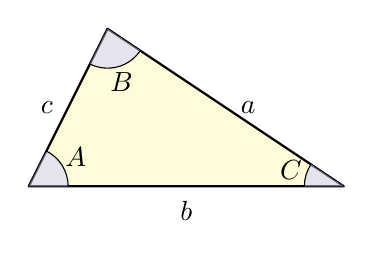
\begin{tikzpicture}
						\tkzDefPoint(0,0){A};
						\tkzDefPoint(1,2){B};
						\tkzDefPoint(4,0){C};
						\tkzDrawPolygon[thick, fill=yellow!15](A,B,C);
						
						\tkzLabelSegment[left=2pt](A,B){$c$};
						\tkzLabelSegment[below=2pt](A,C){$b$};
						\tkzLabelSegment[right=2pt](B,C){$a$}
						
						\tkzFillAngle[size=5mm, fill=blue!20, opacity=0.5](C,A,B);
						\tkzLabelAngle[pos=0.7](C,A,B){$A$};
						\tkzMarkAngle[size=5mm](C,A,B);
						
						\tkzFillAngle[size=5mm, fill=blue!20, opacity=0.5](A,B,C);
						\tkzLabelAngle[pos=0.7](A,B,C){$B$};
						\tkzMarkAngle[size=5mm](A,B,C);
						
						\tkzFillAngle[size=5mm, fill=blue!20, opacity=0.5](B,C,A);
						\tkzLabelAngle[pos=0.7](B,C,A){$C$};
						\tkzMarkAngle[size=5mm](B,C,A);
					\end{tikzpicture}
				\end{minipage}
				\hfill
				\begin{minipage}{0.5\textwidth}
					\centering
						\[
						\frac{\sin A}{a}=\frac{\sin B}{b}=\frac{\sin C}{c}
						\]
						\textbf{OR}
						\[
						\frac{a}{\sin A}=\frac{b}{\sin B}=\frac{c}{\sin C}
						\]
				\end{minipage}
				\begin{Note}
					Side $a$ is always opposite angle $A$, side $b$ is always opposite angle $B$ and side $c$ is always opposite angle $C$.
				\end{Note}
				\paragraph{Proof of the Sine Rule}\mbox{}\\
					\begin{minipage}[t]{0.4\textwidth}
						\vspace{0pt}
						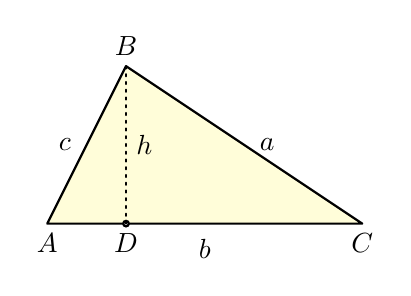
\begin{tikzpicture}
							\tkzDefPoint(0,0){A};
							\tkzDefPoint(1,2){B};
							\tkzDefPoint(4,0){C};
							\tkzDefPoint(1,0){D};
							\tkzDrawPolygon[thick, fill=yellow!15](A,B,C);
							\tkzDrawPoint[thick](D);
							
							\tkzLabelSegment[left=2pt](A,B){$c$};
							\tkzLabelSegment[below=2pt](A,C){$b$};
							\tkzLabelSegment[right=2pt](B,C){$a$};
							
							\tkzLabelPoints[above](B);
							\tkzLabelPoints[below](A,C,D);
							\tkzDrawSegment[thick, dotted](D,B);
							\tkzLabelPoint[right](1,1){$h$};
						\end{tikzpicture}
					\end{minipage}
					\hfill
					\begin{minipage}[t]{0.5\textwidth}
						\vspace{0pt}
						\begin{align*}
							&\text{Consider }\triangle ABD. & \text{Consider }\triangle BCD.\\
							&\sin A=\frac{h}{c} & \sin C=\frac{h}{a}\\
							&\therefore h=c\sin A\;\;\textbf{(1)} & \therefore h=a\sin C\;\;\textbf{(2)} \\
							\\
							&\textbf{(1)}=\textbf{(2)} \therefore c\sin A=a\sin C \\
							&\implies\frac{c}{\sin C}=\frac{a}{\sin A}\;\;\;\text{(Sine rule)} \qed
						\end{align*}
					\end{minipage}
				\paragraph{Two sides and Non-included Angle (Special Case)}\mbox{}\\
					Use the same rule to find the magnitude of $\angle ZXY$ given $\angle Y=25^\circ$, $y=5cm$ and $z=6cm$.\newline
					\begin{minipage}[t]{0.4\textwidth}
						\vspace{0pt}
						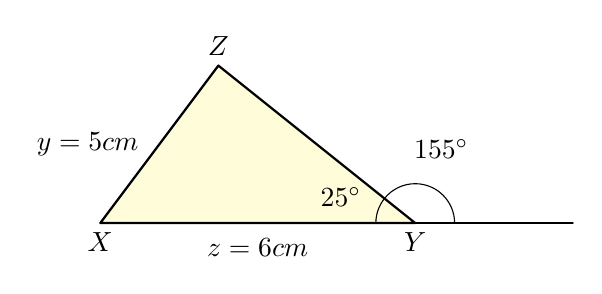
\begin{tikzpicture}
							\tkzDefPoint(0,0){X};
							\tkzDefPoint(1.5,2){Z};
							\tkzDefPoint(4,0){Y};
							\tkzDefPoint(6,0){A};
							\tkzDrawPolygon[thick, fill=yellow!15](X,Y,Z);
							\tkzDrawSegment[thick](Y,A);
							
							\tkzMarkAngle[size=5mm](A,Y,Z);
							\tkzLabelAngle[pos=1](A,Y,Z){$155^\circ$};
							
							\tkzMarkAngle[size=5mm](Z,Y,X);
							\tkzLabelAngle[pos=1](Z,Y,X){$25^\circ$};
							
							\tkzLabelSegment[left=4pt](Z,X){$y=5cm$};
							\tkzLabelSegment[below=2pt](X,Y){$z=6cm$};
							
							\tkzLabelPoints[above](Z);
							\tkzLabelPoints[below](X,Y);
						\end{tikzpicture}
					\end{minipage}
					\hfill
					\begin{minipage}[t]{0.5\textwidth}
						\vspace{0pt}
						\begin{align*}
							&\angle X + \angle Z=155^\circ \\\\
							&\frac{\sin25}{5}=\frac{\sin\angle Z}{6} \implies \angle Z = 30.47^\circ \\
							&\therefore \angle ZXY = 155-30.47=124.53^\circ
						\end{align*}
					\end{minipage}
			\subsubsection{Cosine Rule}
		\subsection{Non-Linear Relations}
			\subsubsection{Parametric Curves}
				A parametric curve in the plane is given by a pair of equations:
				\[
					x=f(t) \text{ and }y=g(t)
				\]
				Where $t$ is called the \textbf{parameter} of the curve.
				\paragraph{Description}
					When asked to describe any parametric curve, you need to consider the direction which a particle following that parametric curve would travel, as well as the point at which the motion starts/ends.
		\subsection{Circles}
			\subsubsection{Equations}
				\bgroup
				\def\arraystretch{2}
				\begin{table}[H]
					\centering
					\begin{tabular}{|c|c|}
						\hline
						\multicolumn{2}{|c|}{\textbf{Circle Equations}} \\
						\hline
						\textit{Cartesian} & \textit{Parametric} \\
						\hline
						$x^2+y^2=r^2$ & {$\!\begin{aligned}x&=r\cos(t)\\y&=r\sin(t)\end{aligned}$} \\
						\hline
					\end{tabular}
				\end{table}
				\egroup
			\subsubsection{Inequalities}
		\subsection{Ellipses}
			\subsubsection{Equations}
			\subsubsection{Inequalities}
		\subsection{Algorithms}
			\subsubsection{Karatsuba's Multiplication Algorithm}
				To find the product of a pair of two-digit numbers $m=10a+b$ and $n=10c+d$.
				\bgroup
				\def\arraystretch{1.5}
				\begin{table}[h]
					\centering
					\begin{tabularx}{\textwidth}{
							|>{\hsize=.1\hsize}X
							>{\hsize=1.9\hsize}X|
						}
						\hline
						\multicolumn{2}{|c|}{\textbf{Karatsuba's Multiplication Algorithm}} \\
						1 & Calculate $ac$. Call the result F. \\
						2 & Calculate $bd$. Call the result G. \\
						3 & Calculate $(a+b)(c+d)$. Call the result H. \\
						4 & Calculate H-F-G. Call the result K. \\
						5 & Calculate 100F+10K+G. The result is $mn$. \\
						\hline
					\end{tabularx}
				\end{table}
				\egroup
				\newline\underline{Example}\newline
				\textit{Use Karatsuba's multiplication algorithm to calculate $23\times31$.}
				\begin{gather*}
					23=2\times10+3,\;31=3\times10+1 \\
					a=2,b=3,c=3,d=1 \\
					ac=2\times3=6=F \\
					bd=3\times1=3=G \\
					(a+b)(c+d)=(2+3)(3+1)=20=H \\
					H-F-G=20-6-3=11=K \\
					mn=100F+10K+G=100(6)+10(11)+3=713
				\end{gather*}
			\subsubsection{Decimal $\to$ Binary}
				Binary uses only the digits 0 and 1 to represent numbers. The positions of digits correspond to different powers of 2.
				\bgroup
				\def\arraystretch{1.5}
				\begin{table}[h]
					\centering
					\begin{tabularx}{\linewidth}{
							|>{\hsize=.1\hsize}X
							>{\hsize=1.9\hsize}X|
						}
						\hline
						\multicolumn{2}{|c|}{\textbf{Algorithm for Decimal to Binary Conversion}} \\
						1 & Input $n$ \\
						2 & Let $q$ be the quotient when $n$ is divided by 2. \\
						3 & Let $r$ be the remainder when $n$ is divided by 2. \\
						4 & Record $r$. \\
						5 & Let $n$ have the value of $q$. \\
						6 & If $n>0$, then repeat from Step 2. \\
						7 & Write the recorded values of $r$ in reverse order. \\
						\hline
					\end{tabularx}
				\end{table}
				\egroup
				\newline\underline{Example}\newline
				\textit{Convert the decimal number 237 into binary form.}
				\begin{gather*}
					n=237, q=118, r=1 \\
					n=118, q=59, r=0 \\
					n=59, q=29, r=1 \\
					n=29, q=14, r=1 \\
					n=14, q=7, r=0 \\
					n=7, q=3, r=1 \\
					n=3, q=1, r=1 \\
					n=1, q=0, r=1 \\
					\therefore237\to11101101
				\end{gather*}
			\subsubsection{The Euclidian Algorithm}
				Can be used to determine the Highest Common Factor (HCF) of a pair of integers.
				\bgroup
				\def\arraystretch{1.5}
				\begin{table}[h]
					\centering
					\begin{tabularx}{\textwidth}{|X|}
						\hline
						\textbf{Euclidean Division} \\
						If $a$ and $b$ are integers with $b>0$, then there are unique integers $q$ and $r$ such that $a=qb+r$ where $0\le r<b$ \\
						\hline
					\end{tabularx}
				\end{table}
				\egroup\\
				\begin{Note}
					Here $q$ is the \textit{quotient} and $r$ is the \textit{remainder} when $a$ is divided by $b$.
				\end{Note}
				\newtheorem*{euclidianDivTheorem*}{Theorem}
				\begin{euclidianDivTheorem*}
					Let $a$ and $b$ be two integers with $b\neq0$. If $a=qb+r$, where $q$ and $r$ are integers, then HCF($a,b$)=HCF($b,r$).
				\end{euclidianDivTheorem*}
				\noindent\underline{Example}\newline
				\textit{Find the highest common factor of 72 and 42.}
				\begin{gather*}
					72=1\times42+30 \\
					HCF(72,42)=HCF(42,30) \\
					42=1\times30+12 \\
					HCF(42,30)=HCF(30,12) \\
					30=2\times12+6 \\
					HCF(30,12)=HCF(12,6)=6 \\
					\therefore HCF(72,42)=6
				\end{gather*}
			\subsubsection{Iteration and Selection}
				\paragraph{Assignment of Values to Variables}\mbox{}\\
					Variables are strings of one or more letters that act as placeholders for different values that can change. Assigning a value to a variable is denoted by a right-to-left arrow ($\leftarrow$). For example, $x\leftarrow3$ means 'assign the value of 3 to variable $x$.'\newline\newline
					Consider the following instructions:\newline
					Step 1: $x\leftarrow3$ \newline
					Step 2: $y\leftarrow2x+1$ \newline
					Step 3: $x\leftarrow4$ \newline
					After following the above steps, we have $x=4$ and $y=7$.
				\paragraph{Iteration}\mbox{}\\
					Iteration is the construction of a loop that allows the controlled repetition of algorithmic steps.\newline\newline
					\newpage
					\noindent\underline{Example}\newline
					\textit{An initial investment of \$100 000 is invested at an interest rate of 5\% p.a. compounded annually.}\newline
					(a) Write an algorithm to find the value of the investment at the end of each year for the first five years.\newline
					\bgroup
					\def\arraystretch{1.5}
					\begin{table}[h]
						\centering
						\begin{tabular}{|l|l|}
							\hline
							1 & $V\gets 000$ and $n\gets$. \\
							2 & Print $n$ and Print $V$. \\
							3 & $V\gets V\times1.05$ and $n\gets n+1$. \\
							4 & Print $n$ and Print $V$ \\
							5 & Repeat from step 3 while $n<5$. \\
							\hline
						\end{tabular}
					\end{table}
					\egroup
					\newline
					(b) Demonstrate the algorithm with a table of values.\newline
					\bgroup
					\def\arraystretch{1.5}
					\begin{table}[h]
						\centering
						\begin{tabular}{|l|c|}
							\hline
							n & V \\
							0 & 100 000 \\ 
							1 & 105 000 \\
							2 & 110 250 \\
							3 & 115 762.5 \\
							4 & 121 550.63 \\
							5 & 127 628.16 \\
							\hline
						\end{tabular}
					\end{table}
					\egroup
				\paragraph{Selection}\mbox{}\\
					Decision-making constructs allow us to specify whether certain steps should be followed based on some condition. For example, we can use an instruction such as 'If... then...". This is called selection.
					\newpage
					\noindent\underline{Example}\newline
					\[
						\text{For }n\in\mathbb{N},\text{ define }t_n=\begin{cases}
							2n+4 & \text{if n is even} \\
							n+3 & \text{if n is odd}
						\end{cases}
					\]
					\textbf{(a)} Write an algorithm to generate the first $N$ terms of this sequence.
					\bgroup
					\def\arraystretch{1.5}
					\begin{table}[h]
						\centering
						\begin{tabular}{|l|l|}
							\hline
							1 & $n\gets$ \\
							2 & If $n$ is even, $t\gets+4$. Otherwise, $t\gets n+3$ \\
							3 & Print $n$ and Print $t$. \\
							4 & $n\gets n+1$ \\
							5 & Repeat steps 2 to 4 while $n<N$. \\
							\hline
						\end{tabular}
					\end{table}
					\egroup
					\newline\textbf{(b)} Demonstrate the algorithm for N=6 with a table of values.
					\bgroup
					\def\arraystretch{1.5}
					\begin{table}[h]
						\centering
						\begin{tabular}{|l|c|}
							\hline
							n & t \\
							\hline
							1 & 4 \\
							2 & 8 \\
							3 & 6 \\
							4 & 12 \\
							5 & 8 \\
							6 & 16 \\
							\hline
						\end{tabular}
					\end{table}
					\egroup
			\subsubsection{Pseudocode}
				\paragraph{If-Then Block}\mbox{}\\
					This construct provides a means of making decisions within an algorithm. Certain instructions are only followed if a given condition is satisfied.\newline\newline
					The basic template for an If-Then block is as follows:
					\begin{algorithmic}
						\If{\textit{condition}}
							\State{follow these instructions}
						\EndIf
					\end{algorithmic}
					\underline{Example}\newline
					Using pseudocode, write an algorithm to find the maximum of two numbers $a$ and $b$.\newline
					\begin{algorithmic}
						\State{input $a,b$}
						\If{$a\geq b$}
							\State{print $a$}
						\Else
							\State{print $b$}
						\EndIf
					\end{algorithmic}
				\paragraph{The For Loop}\mbox{}\\
					This construct provides a means of repeatedly executing the same set of instructions in a controlled way.
					\begin{algorithmic}
						\For{condition}
							\State{follow these instructions}
						\EndFor
					\end{algorithmic}\mbox{}\\
					\underline{Example}\newline
					Consider the sequence: $1^2,2^2,3^2,4^2,...,n^2$.\newline
					Using pseudocode, write an algorithm to calculate:\newline\newline
					\textbf{(a)} the sum of the terms in this sequence.
					\begin{algorithmic}
						\State{input $n$}
						\State{sum$\gets0$}
						\For{$i$ from 1 to $n$}
							\State{sum$\gets$sum+$i^2$}
							\State{print sum}
						\EndFor
					\end{algorithmic}\mbox{}\\
					\textbf{(b)} the product of the terms in this sequence.
					\begin{algorithmic}
						\State{input $n$}
						\State{product$\gets1$}
						\For{$i$ from 1 to $n$}
							\State{product$\gets$product$\times i^2$}
							\State{print product}
						\EndFor
					\end{algorithmic}\mbox{}\\
				\paragraph{While Loop}\mbox{}\\
					This construct provides another means of controlled, repeated execution of instructions. It does this by performing iterations indefinitely, as long as some condition remains true.
					\begin{algorithmic}
						\While{condition}
							\State{perform these instructions}
						\EndWhile
					\end{algorithmic}\mbox{}\\
					\underline{Example}\newline
					Consider the sequence defined by the rule:\newline
					$x_{n+1}=5x_n+4,$ where $x_1=3$.\newline
					Write an algorithm that will determine the smallest value of $n$ for which $x_n>10 000$.\marginnote[left]{A \textit{desk check} is a manual verification of the algorithm's function with a table of values.} Show a desk check to test the operation of the algorithm.\newline
					\begin{minipage}{0.45\textwidth}
						\begin{algorithmic}
							\State{$n\gets1$}
							\State{$x\gets3$}
							\While{$x\leq100$}
							\State{$n\gets n+1$}
							\State{$x\gets 5x+4$}
							\EndWhile
							\State{print $n$ and print $x$}
						\end{algorithmic} 
					\end{minipage}\hfill
					\begin{minipage}{0.55\textwidth}
						\begin{tabular}{|l|c|}
							\hline
							n & $x_n$ \\
							1 & 3 \\
							2 & 19 \\
							3 & 99 \\
							4 & 499 \\
							5 & 2499 \\
							6 & 12499 \\
							\hline
						\end{tabular}
					\end{minipage}
				\paragraph{Functions}\mbox{}\\
					A function takes one or more input values and returns an output value. Functions can be defined and then used in other algorithms.\newline\newline
					\underline{Example}\newline
					Define the function $f(x)=3x+2$.\newline
					\textbf{define} f(x):\newline
					\-\hspace{1em}$y\gets 3x+2$\newline
					\-\hspace{1em}return $y$
					\subparagraph{The Quotient and Remainder Functions}\mbox{}\\
		\subsection{Complex Numbers}
			\subsubsection{Definition}
				\paragraph{Imaginary Numbers}\mbox{}\\
					The imaginary number $i$ has the property that $i^2=-1$. By declaring $i=\sqrt{-1}$ we can find square roots of all negative numbers.
					\begin{align*}
						\sqrt{-4}&=\sqrt{4\times(-1)} \\ &=\sqrt{4}\times\sqrt{-1} \\ &=2i
					\end{align*}
				\paragraph{Complex Numbers}\mbox{}\\
					A complex number is an expression in the form $a+bi$ where $a,b\in\mathbb{R}$ and $i=\sqrt{-1}$.
					\marginnote[left]{The Imaginary Part of a complex number is the \textit{coefficient} of i \textbf{only}. Do not include $i$ when stating the imaginary part.}
					\begin{equation*}
						\begin{aligned}
							\text{Let }z=a+bi,\;a,b\in\mathbb{R}\\
							\text{Real Part: }Re(z)=a \\
							\text{Imaginary Part: }Im(z)=b \\
						\end{aligned}
					\end{equation*}
			\subsubsection{Equality of Complex Numbers}
				\begin{equation*}
					\begin{aligned}
						\text{Let }z_1=a+bi\text{ and }z_2=c+di,\;a,b,c,d\in\mathbb{R}. \\
						\text{If }z_1=z_2,\text{ then }a=c, b=d
					\end{aligned}
				\end{equation*}
			\subsubsection{Argand Diagram}
				\begin{minipage}[t]{0.6\textwidth}
					\vspace{0pt}
					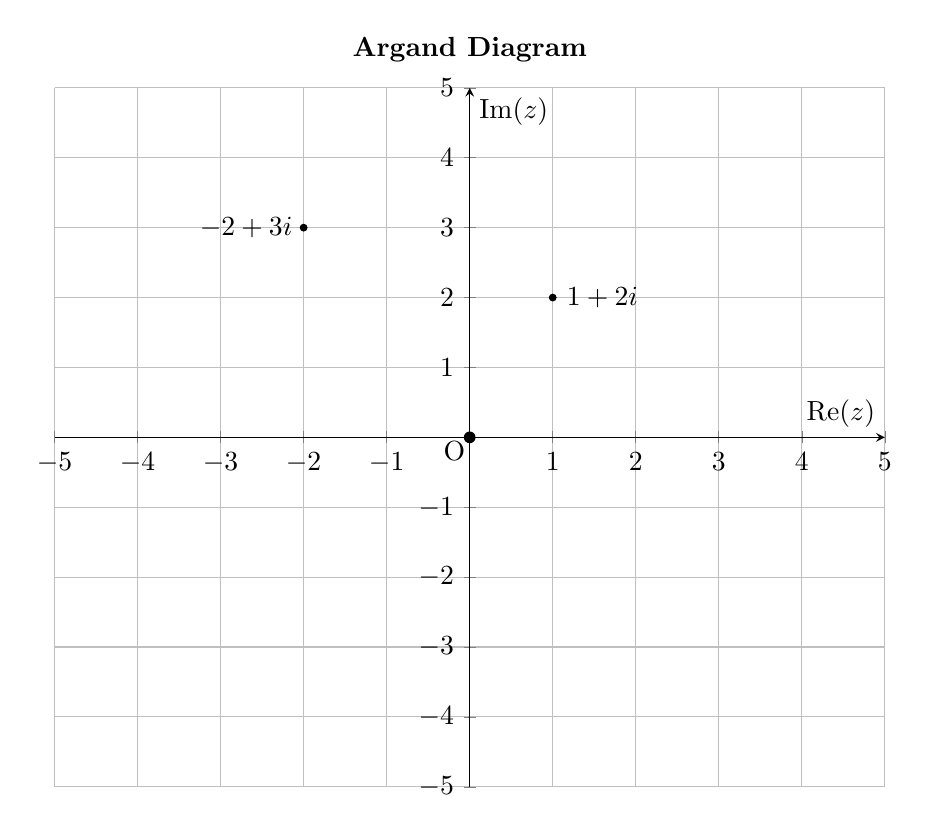
\begin{tikzpicture}
						
						\begin{axis}
							[
							title=\textbf{Argand Diagram},
							xmin=-5,
							xmax=5,
							xtick distance={1},
							ymin=-5,
							ymax=5,
							ytick distance={1},
							axis lines=middle,
							grid,
							xlabel=Re$(z)$,
							ylabel=Im$(z)$			
							]
							\node[label={[label distance=-5]225:{O}}, circle, fill, inner sep=1.5pt,] at (axis cs:0,0) {};
							
							\node[label={0:{$1+2i$}},circle, fill, inner sep=1pt] at (axis cs:1,2) {};
							\node[label={[xshift=-1.5cm]0:{$-2+3i$}},circle, fill, inner sep=1pt] at (axis cs:-2,3) {};
						\end{axis}
					\end{tikzpicture}
				\end{minipage}\hfill
				\begin{minipage}[t]{0.4\textwidth}
					\vspace{0pt}
					\centering
					An Argand Diagram is a geometric representation of the set of complex numbers. In a vector sense, a complex number has two dimensions: the real and the imaginary parts. Therefore a plane is required to represent $\mathbb{C}$.\newline\newline
					The horizontal axis represents Re($z$) for $z\in\mathbb{C}$, and the vertical axis represents Im($z$), for $z\in\mathbb{C}$.\newline\newline
					A complex number $a+bi$ is at the point $(a,b)$ on the Argand Diagram. A complex number in the form $a+bi$ is said to be in \textbf{cartesian form}.
				\end{minipage}
				\paragraph{Geometric Representations of Basic Operations}\mbox{}\\
					\textit{Addition}\newline
					\begin{minipage}[t]{0.6\textwidth}
						\vspace{0pt}
						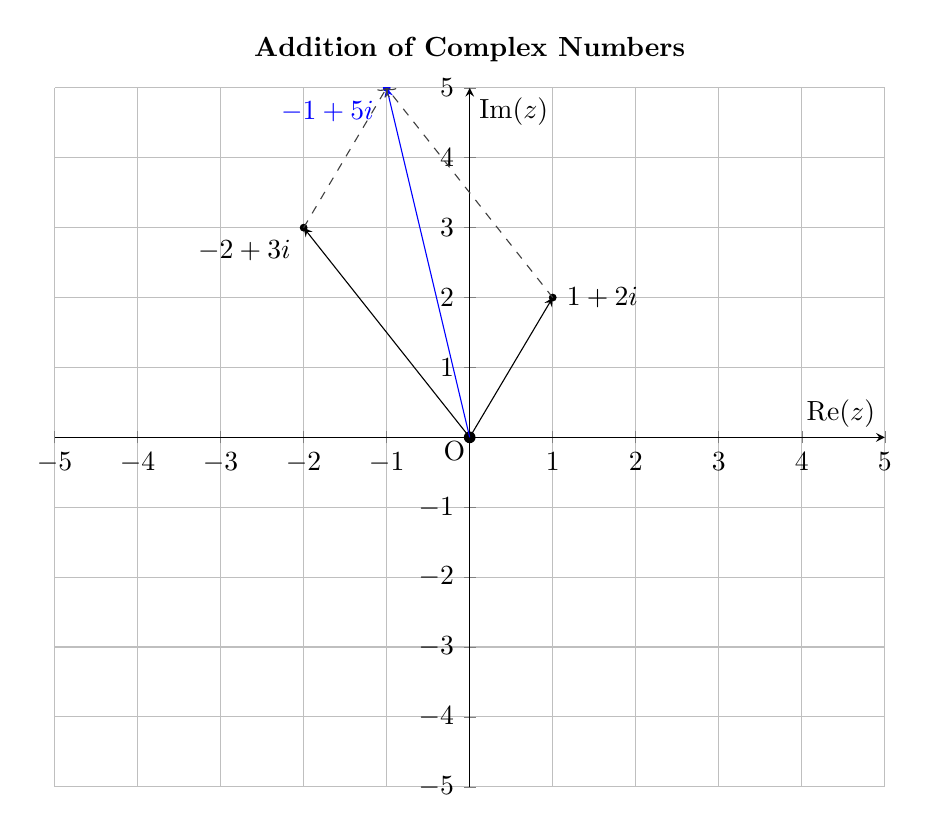
\begin{tikzpicture}
							
							\begin{axis}
								[
								title=\textbf{Addition of Complex Numbers},
								xmin=-5,
								xmax=5,
								xtick distance={1},
								ymin=-5,
								ymax=5,
								ytick distance={1},
								axis lines=middle,
								grid,
								xlabel=Re$(z)$,
								ylabel=Im$(z)$			
								]
								\node[label={[label distance=-5]225:{O}}, circle, fill, inner sep=1.5pt,] at (axis cs:0,0) {};
								
								\draw [thin,>=stealth] (axis cs:0,0) [->](0,0) -- (1,2);
								\node[label={0:{$1+2i$}},circle, fill, inner sep=1pt] at (axis cs:1,2) {};
								
								\draw [thin, >=stealth] (axis cs:0,0) [->](0,0) -- (-2,3);
								\node[label={225:{$-2+3i$}},circle, fill, inner sep=1pt] at (axis cs:-2,3) {};
								
								\draw [thin, >=stealth, blue] (axis cs:0,0) [->](0,0) -- (-1,5);
								\node[label={[text=blue]225:{$-1+5i$}},circle, fill, inner sep=1pt, blue] at (axis cs:-1,5) {};
								
								\draw [dashed, thin, darkgray] (axis cs:1,2) [->](1,2) -- (-1,5);
								\draw [dashed, thin, darkgray] (axis cs:-2,3) [->](-2,3) -- (-1,5);

							\end{axis}
						\end{tikzpicture}
					\end{minipage}\hfill
					\begin{minipage}[t]{0.4\textwidth}
						\centering
						Addition of complex numbers on an Argand Diagram acts like vector addition. To do this, you form a parallelogram with the two complex numbers and the origin. The fourth point is the sum of the two complex numbers. This is illustrated to the left.
					\end{minipage}
					\newpage
					\textit{Scalar Multiplication}\newline
					\begin{minipage}[t]{0.6\textwidth}
						\vspace{0pt}
						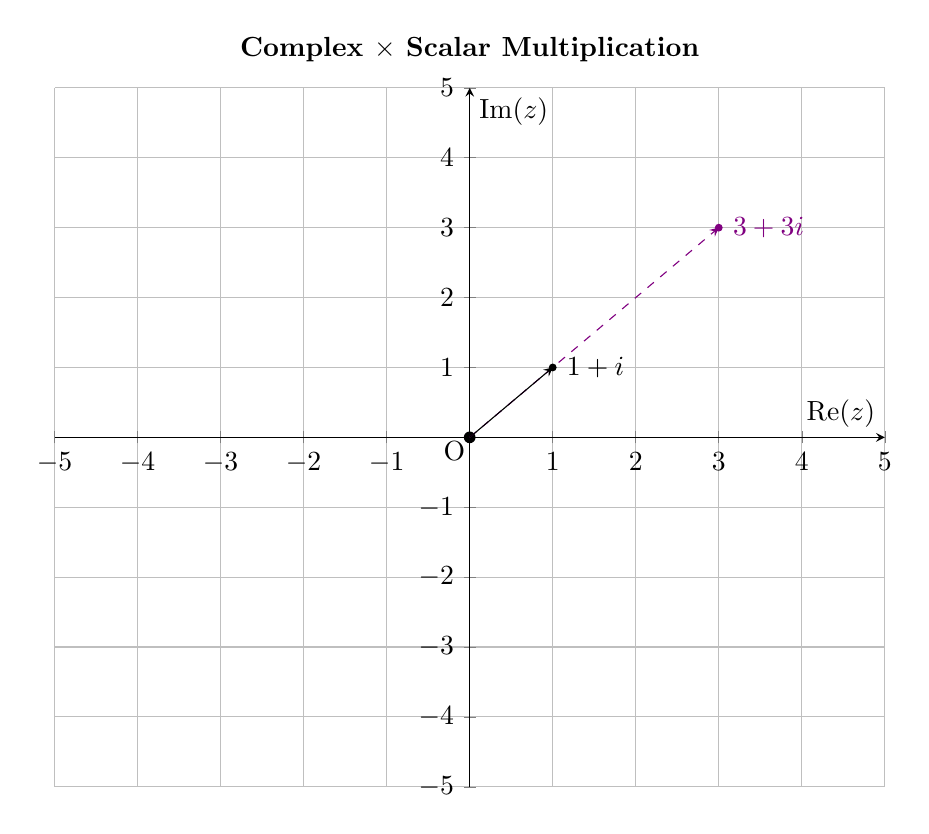
\begin{tikzpicture}
							
							\begin{axis}
								[
								title=\textbf{Complex $\times$ Scalar Multiplication},
								xmin=-5,
								xmax=5,
								xtick distance={1},
								ymin=-5,
								ymax=5,
								ytick distance={1},
								axis lines=middle,
								grid,
								xlabel=Re$(z)$,
								ylabel=Im$(z)$			
								]
								\node[label={[label distance=-5]225:{O}}, circle, fill, inner sep=1.5pt,] at (axis cs:0,0) {};
								
								\draw [dashed, violet, >=stealth] (axis cs:0,0) [->] (0,0) -- (3,3);
								\node[label={[text=violet]0:{$3+3i$}}, circle, violet, fill, inner sep=1pt] at (axis cs:3,3) {};
								
								\draw [thin,>=stealth] (axis cs:0,0) [->](0,0) -- (1,1);
								\node[label={0:{$1+i$}}, circle, fill, inner sep=1pt] at (axis cs:1,1) {};
							\end{axis}
						\end{tikzpicture}
					\end{minipage}
					\hfill
					\begin{minipage}[t]{0.4\textwidth}
						\vspace{0pt}
						Multiplying a complex number by a scalar $k$ extends the distance of the complex number from the origin on the Argand Diagram by a factor of $k$.
						\newline\newline
						You can draw a straight line through $z$, $kz$, and the origin.
						\newline\newline
						The Argand Diagram on the left shows the multiplication of $z=1+i$ by a factor of $k=3$.
					\end{minipage}
				\paragraph{Multiplication by $i$}\mbox{}\\
					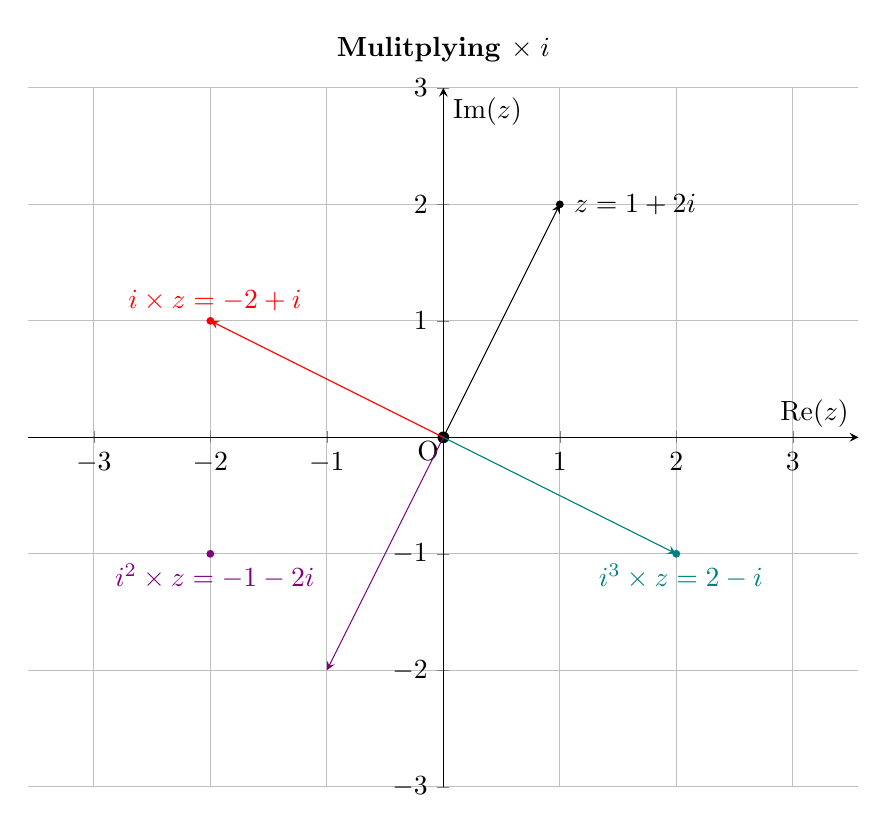
\begin{tikzpicture}
						
						\begin{axis}
							[
							title=\textbf{Mulitplying $\times\;i$},
							xmin=-3,
							xmax=3,
							xtick distance={1},
							ymin=-3,
							ymax=3,
							ytick distance={1},
							axis lines=middle,
							grid,
							xlabel=Re$(z)$,
							ylabel=Im$(z)$,
							axis equal		
							]
							\node[label={[label distance=-5]225:{O}}, circle, fill, inner sep=1.5pt,] at (axis cs:0,0) {};
							
							\draw [thin, >=stealth] (axis cs:0,0) [->] (0,0) -- (1,2);
							\node[label=0:{$z=1+2i$}, circle, fill, inner sep=1pt] at (axis cs:1,2) {};
							
							\draw [thin, red, >=stealth] (axis cs:0,0) [->] (0,0) -- (-2,1);
							\node[label={[text=red, above]0:{$i\times z=-2+i$}}, circle, red, fill, inner sep=1pt] at (axis cs:-2,1) {};
							
							\draw [thin, violet, >=stealth] (axis cs:0,0) [->] (0,0) -- (-1,-2);
							\node [label={[text=violet, below]0:{$i^2\times z=-1-2i$}}, circle, violet, fill, inner sep=1pt] at (axis cs:-2,-1){};
							
							\draw [thin, teal, >=stealth] (axis cs:0,0) [->] (0,0) -- (2,-1);
							\node [label={[text=teal, below]0:{$i^3\times z=2-i$}}, circle, teal, fill, inner sep=1pt] at (axis cs:2,-1){};
 						\end{axis}
					\end{tikzpicture}\mbox{}\\
					By multiplying by $i$, a complex number is rotated 90$^\circ$ counterclockwise through the Argand Diagram about the origin. \textbf{Distance from the origin is conserved.}
			\subsubsection{Addition, Multiplication of Complex Numbers}
				\[
					\text{Let }z_1=a+bi,\;z_2=c+di
				\]
				\paragraph{Addition}\mbox{}\\
					\[
						z_1+z_2=(a+c)+(b+d)i
					\]
				\paragraph{Subtraction}\mbox{}\\
					\[
						z_1-z_2=(a-c)+(b-d)i
					\]
				\paragraph{Multiplication by a real constant}\mbox{}\\
					\[
						kz_1=k(a+bi)=ka+kbi
					\]
				\underline{Example}\newline
				Evaluate:\newline
				\begin{minipage}[t]{0.5\textwidth}
					(a) $(2-5i)+(-4+3i)$
					\begin{align*}
						&=(2-4)+(-5+3)i \\
						&=-2-2i \\
						&=-2(1-i)
					\end{align*}
				\end{minipage}
				\hfill
				\begin{minipage}[t]{0.5\textwidth}
					(b) $5(5-3i)-(2-i)$
					\begin{align*}
						&=(25-15i)-(2-i) \\
						&=(25-2)+(-15+1)i \\
						&=23-14i
					\end{align*}
				\end{minipage}
				\paragraph{Multiplication of Complex Numbers}\mbox{}\\
					\begin{minipage}[t]{0.2\textwidth}
						\begin{align*}
							(a+bi)(c+di)&=ac+adi+bci+bdi^2 \\
							&=(ac-bd)+(bc+ad)i
						\end{align*}
					\end{minipage}
					\hfill
					\begin{minipage}[t]{0.5\textwidth}
						\underline{Example}
						\begin{align*}
							(5+2i)(3-4i)&=(5\times3-2\times(-4))+(2\times3+5\times(-4))i \\
							&=(15+8)+(6-20)i=23-14i
						\end{align*}
					\end{minipage}
				\paragraph{Powers of $i$}\mbox{}\\
					$i^{4n}=1,\;i^{4n+1}=i,\;i^{4n+2}=-1,\;i^{4n+3}=-i$
				\paragraph{The Sum of Two Squares}\mbox{}\\
					\begin{align*}
						i^2=-1\\
						\therefore a^2+b^2&=a^2-i^2b^2 \\
						&=a^2-(bi)^2 \\
						&=(a+bi)(a-bi)
					\end{align*}
			\subsubsection{Conjugates}
				If $z=a+bi$ then it's conjugate is $\overline{z}=a-bi$. \newline
				\begin{table}[H]
					\centering
					\bgroup
					\def\arraystretch{1.5}
					\begin{tabular}{|c|}
						\hline
						\textbf{Properties of Conjugates} \\
						\hline
						$z\overline{z}=|z|^2$ \\
						\hline
						$\overline{z_1+z_2}=\overline{z_1}+\overline{z_2}$ \\
						\hline
						$\overline{z_1z_2}=\overline{z_1}\times\overline{z_2}$ \\
						\hline
						$\overline{kz}=k\overline{z}$ \\
						\hline
						$z+\overline{z}=2Re(z)$ \\
						\hline
					\end{tabular}
					\egroup
				\end{table}\mbox{}\\
				\underline{Example}\newline
				Let $z_1=3+2i$ and $z_2=5-3i$ \newline\newline
				\begin{minipage}[t]{0.4\textwidth}
					(a) Show that $\overline{z_1+z_2}=\overline{z_1}+\overline{z_2}$
					\begin{align*}
						z_1+z_2&=(3+2i)+(5-3i)\\
						&=8-i \\
						&\text{\underline{LHS}}\\
						\overline{z_1+z_2}&=\overline{8-i} \\
						&=8+i \\
						&\text{\underline{RHS}}\\
						\overline{z_1}&=3-2i \\
						\overline{z_2}&=5+3i \\
						\overline{z_1}+\overline{z_2}&=8+i=\text{LHS}\qed
					\end{align*}
				\end{minipage}
				\hfill
				\begin{minipage}[t]{0.4\textwidth}
					(b) Show that $\overline{z_1\times z_2}=\overline{z_1}\times\overline{z_2}$
					\begin{align*}
						z_1\times z_2&=(3+2i)\times(5-3i) \\
						&=(15+6)+(10-9)i\\
						&=21+i\\
						\therefore\text{\underline{LHS}}&=\overline{21+i}=21-i \\
						&\text{\underline{RHS}} \\
						\overline{z_1}&=3-2i \\
						\overline{z_2}&=5+3i \\
						\therefore\text{\underline{RHS}}&=(15+6)+(-10+9)i \\
						&=21-i=\text{RHS}\qed
					\end{align*}
				\end{minipage}
			\subsubsection{Division of Complex Numbers}
				\[
					\frac{3+2i}{i}\times\frac{i}{i}=\frac{(3+2i)i}{-1}=\frac{3i-2}{-1}=2-3i
				\]
				In the above example, by multiplying the division of the two complex numbers by $\frac{i}{i}$, you make the denominator real, hence allowing us to find the quotient.
				\[
					\frac{4+2i}{3-2i}\times\frac{3+2i}{3+2i}=\frac{12+8i+6i+4i^2}{9+4}=\frac{8+14i}{13}=\frac{8}{13}+\frac{14}{13}i
				\]
				In the above example, we multiply both the numerator and denominator by the conjugate of the denominator. This makes the denominator a real number, allowing us to simplify the complex division.\newline\newline
				\underline{Example}\newline
				Solve for $z$: $(2-i)z=42i$\newline
				\begin{align*}
					z&=\frac{42i}{2-i} \\
					&=\frac{42i}{2-i}\times\frac{2+i}{2+i} \\
					&=\frac{84i+42i^2}{4+1}=\frac{84i-42}{5} \\
					z&=-\frac{42}{5}+\frac{84}{5}i \;\;\;\;\checkmark
				\end{align*}
			\subsubsection{Polar Form}
				\paragraph{Polar Coordinates}\mbox{}\\
					Consider the point $P(x,y)$ on the cartesian plane. The point $P$ always makes a distance $r$ from the origin and an angle $\theta$ from the positive x-axis.\newline
					\begin{minipage}[t]{0.6\textwidth}
						\vspace{0pt}
						\begin{tikzpicture}
							\begin{axis} [xmin=-5, xmax=5, ymax=5, ymin=-2, axis lines=middle,xlabel=$x$, ylabel=$y$, title={\textbf{Cartesian Plane}}, xticklabels={,,}, yticklabels={,,}]
								\draw [thin] (axis cs:0,0) (0,0) -- (3,3);
								\node [label={[above=5]0:{$r$}}] at (axis cs:1.5,1.5){};
								
								\begin{scope}
									\path[clip] (0,0) -- (2,0) -- (2,2);
									\fill[gray, opacity=0.5, draw=black] (0,0) circle (5mm);
									\node at ($(0,0)+(20:7mm)$) {$\theta$};
								\end{scope}
							
								\draw [dotted] (axis cs:0,-0.1) (0,-0.1) -- (3,-0.1);
								\node [label={[below=5]0:{$x$}}] at (axis cs: 1.5,0){};
								
								\draw[dotted] (axis cs:3,0) (3,0) -- (3,3);
								\node [label={[right]0:{$y$}}] at (axis cs: 3,1.5){};
							\end{axis}
						\end{tikzpicture}
					\end{minipage}
					\hfill
					\begin{minipage}[t]{0.4\textwidth}
						\vspace{0pt}
						\begin{align*}
							&\cos(\theta)=\frac{x}{r}\implies x=r\cos(\theta) \\
							&\sin(\theta)=\frac{y}{r}\implies y=r\sin(\theta) \\
							&\tan(\theta)=\frac{y}{x} \\
							&r=\sqrt{x^2+y^2}
						\end{align*}
					\end{minipage}
					\underline{Example}\newline
					Convert the following cartesian coordinates into polar form.\newline
					\begin{minipage}[t]{0.5\textwidth}
						(a) A(2,2) \newline
						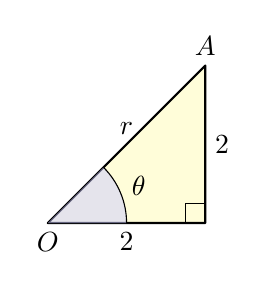
\begin{tikzpicture}
							
							\tkzDefPoint(0,0){O};
							\tkzDefPoint(2,2){A};
							\tkzDefPoint(2,0){B};
							\tkzLabelPoints[above](A);
							\tkzLabelPoints(O);
							\tkzDrawPolygon[thick, fill=yellow!15](O,A,B);
							
							\tkzFillAngle[fill=blue!20, opacity=0.5](B,O,A);
							\tkzLabelAngle[pos=1.25](B,O,A){$\theta$};
							\tkzMarkAngle(B,O,A);
							\tkzMarkRightAngle(A,B,O);
							
							\tkzLabelLine[pos=0.5,below,](O,B){2};
							\tkzLabelLine[pos=0.5,right,](B,A){2};
							\tkzLabelLine[pos=0.5,above,](O,A){$r$};
						\end{tikzpicture}\mbox{}\\
						\begin{align*}
							&r=\sqrt{2^2+2^2}=\sqrt{8}=2\sqrt{2} \\
							&\tan(\theta)=\frac{2}{2}=1\therefore \theta=\frac{\pi}{4}^c \\
							&\therefore A(2\sqrt{2},\frac{\pi}{4}^c)
						\end{align*}
					\end{minipage}
					\hfill
					\begin{minipage}[t]{0.5\textwidth}
						(b) B(-1, $\sqrt{3}$)\newline
						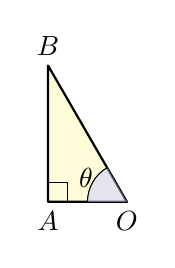
\begin{tikzpicture}
							\tkzDefPoint(0,0){O};
							\tkzDefPoint(-1,0){A};
							\tkzDefPoint(-1,1.73){B};
							\tkzLabelPoints[above](B);
							\tkzLabelPoints(O,A);
							\tkzDrawPolygon[thick, fill=yellow!15](O,B,A);
							
							\tkzFillAngle[size=0.5, fill=blue!20, opacity=0.5](B,O,A);
							\tkzLabelAngle[pos=0.6](B,O,A){$\theta$};
							\tkzMarkAngle[size=0.5](B,O,A);
							\tkzMarkRightAngle(B,A,O);
						\end{tikzpicture}\mbox{}\\
						\begin{align*}
							&r=\sqrt{(-1)^2+(\sqrt{3})^2}=\sqrt{4}=2 \\
							&\tan(\theta)=\frac{\sqrt{3}}{-1}=-\sqrt{3} \\
							&\therefore Base\;Angle=\frac{\pi}{3} \therefore \theta=\frac{2\pi}{3} \\
							&\therefore B(2,\frac{2\pi}{3}^c)
						\end{align*}
					\end{minipage}
				\paragraph{The Polar Plane}\mbox{}\\
					\begin{minipage}[t]{0.5\textwidth}
						\vspace{0pt}
						content
					\end{minipage}
					\hfill
					\begin{minipage}[t]{0.5\textwidth}
						\vspace{0pt}
						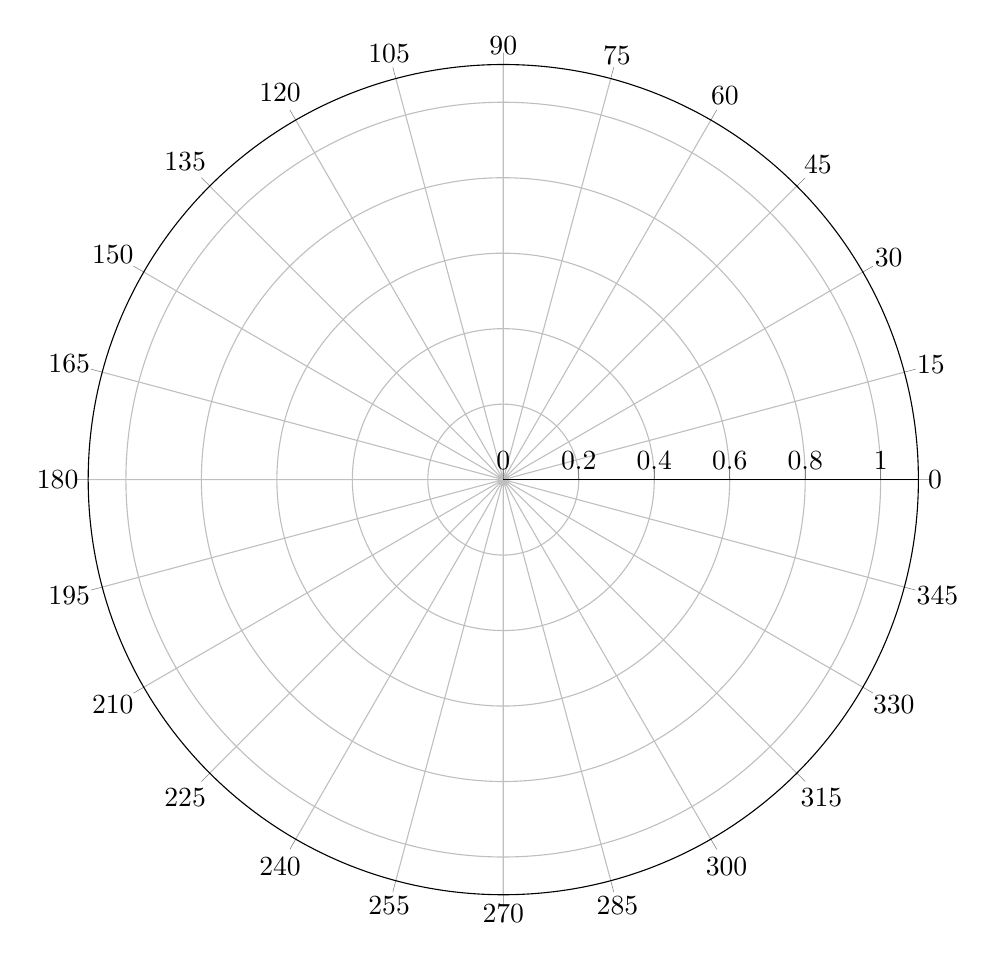
\begin{tikzpicture}
							\begin{polaraxis}
								
							\end{polaraxis}
						\end{tikzpicture}
					\end{minipage}
				\paragraph{Polar Form of Complex Numbers}\mbox{}\\
					A complex number of form $z=a+bi$ is said to be in \textbf{cartesian form}. This can be converted to polar form as follows:\newline
					\marginnote[left]{$r=|z|=\sqrt{a^2+b^2}$\newline\newline$\theta=\Arg(z)=\arctan\left(\frac{b}{a}\right)$}
					\begin{align*}
						z&=a+bi \\
						\text{On an Argand Diagram, }&a=r\cos\theta\text{ and }b=r\sin\theta. \\
						\therefore z&=r\cos\theta+r\sin\theta i \\
						&=r(\cos\theta+i\sin\theta) \\
						&=r\cis\theta \text{ (Polar Form)} \\
					\end{align*}
					\textit{Principle Value of Argument}\newline
					$\Arg(z)\in(-\pi,\pi]$\newline\newline
					\underline{Example}\newline
					Express the following complex numbers in polar form.\newline
					\begin{minipage}[t]{0.5\textwidth}
						\vspace{0pt}
						(a) $z=1+\sqrt{3}i$\newline
						\begin{align*}
							r&=\sqrt{(1)^2+(\sqrt{3})^2} \\
							&=2=|z| \\
							\\
							\tan\theta&=\frac{\sqrt{3}}{1} \\
							\theta&=\frac{\pi}{3} \\
							\therefore z&=2\cis\left(\frac{\pi}{3}\right)
						\end{align*}
					\end{minipage}
					\hfill
					\begin{minipage}[t]{0.5\textwidth}
						\vspace{0pt}
						(b) $z=2-2i$\newline
						\begin{align*}
							r&=\sqrt{2^2+(-2)^2} \\
							&=\sqrt{8}=2\sqrt{2}=|z| \\
							\\
							\tan\theta&=\frac{-2}{2}=-1 \\
							\theta&=\frac{-\pi}{4} \\
							\therefore z&=2\sqrt{2}\cis\left(\frac{-\pi}{4}\right)
						\end{align*}
					\end{minipage}
					\underline{Example}\newline
					Express $z=2cis\left(\frac{-2\pi}{3}\right)$ in cartesian form.\newline
					\begin{align*}
						|z|&=2=\sqrt{a^2+b^2} && z=a+bi \\
						z&=2\left( \cos\left(\frac{-2\pi}{3}\right) + i\sin\left(\frac{-2\pi}{3}\right) \right) \\
						z&=2(-\frac{1}{2}+i\frac{-\sqrt{3}}{2}) \\
						z&=-1-\sqrt{3}i
					\end{align*}
			\subsubsection{Multiplication and Division in Polar Form}
				If $z_1=r_1\cis\theta_1$ and $z_2=r_2\cis\theta_2$ \newline\newline
				Then $z_1\times z_2 = r_1\times r_2\times\cis(\theta_1+\theta_2)$ \newline\newline and $\frac{z_1}{z_2}=\frac{r_1}{r_2}\times\cis(\theta_1-\theta_2)$.
				\newline\newline
				\underline{Example}\newline
				If $z_1=3\cis\left(\frac{\pi}{2}\right),\;z_2=2\cis\left(\frac{5\pi}{6}\right)$, find $z_1z_2$ in polar form.
				\begin{align*}
					z_1z_2=(3\times2)\times\cis\left(\frac{\pi}{2}+\frac{5\pi}{6}\right)=6\cis\left(\frac{4\pi}{3}\right)=6\cis\left(\frac{-2\pi}{3}\right)
				\end{align*}
				\newpage
				\noindent\underline{Example}\newline
				If $z_1=-\sqrt{3}+i$ and $z_2=2\sqrt{3}+2i$, find $\frac{z_1}{z_2}$ in polar form.
				\begin{align*}
					\frac{z_1}{z_2}&=\frac{-\sqrt{3}+i}{2\sqrt{3}+2i}\times\frac{2\sqrt{3}-2i}{2\sqrt{3}-2i} \\
					&=\frac{-2\times3+2\sqrt{3}i+2\sqrt{3}i+2}{(2\sqrt{3})^2-(2i)^2} \\
					&=\frac{-4+4\sqrt{3}i}{12+4}=\frac{-1+\sqrt{3}i}{4}
				\end{align*}
			\subsubsection{de Moivre's (de Movies) Theorem}
				\begin{align*}
					\text{Let }z&=r\cis\theta \\
					\therefore z^2&=r\cis\theta\times r\cis\theta \\
					&=r^2\cis(2\theta) \\
					\therefore z^3&=r^3\cis(3\theta) \\
					\therefore z^5&=r^5\cis(5\theta) \\
					\ldots
					\\
					&z^n=r^n\cis(n\theta)\text{ (de Moivre's Theorem)}
				\end{align*}
				\underline{Example}\newline
				Evaluate $(2\sqrt{3}-2i)^7$. Give your answer in \textbf{cartesian form}.
				\begin{align*}
					r&=\sqrt{(2\sqrt{3})^2+(2)^2}=\sqrt{4} \\
					\cos\theta&=\frac{2\sqrt{3}}{4}\;\therefore\theta=\frac{\pi}{6} \\
					\sin\theta&=\frac{-1}{2}\;\therefore\theta=-\frac{\pi}{6} \\
					&\therefore\theta=-\frac{\pi}{6} \\
					z&=4\cis\left(-\frac{\pi}{6}\right) \\
					z^7&=4^7\cis\left(-\frac{7\pi}{6}\right) \\
					&=16384\cis\left(\frac{5\pi}{6}\right) \\
					&=16384\left[\cos\left(\frac{5\pi}{6}\right)+i\sin\left(\frac{5\pi}{6}\right)\right]=16384\left[-\frac{\sqrt{3}}{2}+\frac{1}{2}i\right] \\
					&=-8192\sqrt{3}+8192i
				\end{align*}
			\subsubsection{Factorisation of Polynomials}
				\paragraph{Complex Quadratics}\mbox{}\\
					\underline{Example}\newline
					Solve for $z$.\newline
					\begin{minipage}[t]{0.5\textwidth}
						(a)$2z^2+5z+4=0$
						\begin{align*}
							z&=\frac{-b\pm\sqrt{b^2-4ac}}{2a}=\frac{-5\pm\sqrt{-7}}{4}\\
							&=\frac{-5\pm\sqrt{7}i}{4} \\\\
							&\text{Alternatively...}\\
							2z^2+5x+4&=0 \\
							&2\left[z^2+\frac{5}{2}z+2\right]=0 \\
							&2\left[\left(z+\frac{5}{4}\right)^2-\frac{25}{16}+2\right]=0\\
							&2\left[\left(z+\frac{5}{4}\right)^2+\frac{7}{16}\right]=0\\
							&2\left(z+\frac{5}{4}\right)^2+\frac{14}{16}=0 \\
							&\left(z+\frac{5}{4}\right)^2+\frac{7}{16}=0 \\
							&\left(z+\frac{5}{4}\right)^2=-\frac{7}{16} \\
							&z+\frac{5}{4}=\pm\frac{i\sqrt{7}}{4} \\
							&z=-\frac{5}{4}\pm\frac{i\sqrt{7}}{4} \\
							&z=\frac{-5\pm\sqrt{7}i}{4}
						\end{align*}
					\end{minipage}
					\hfill
					\begin{minipage}{0.5\textwidth}
						(b)$z^2-6z+14=0$
						\begin{align*}
							z&=\frac{-b\pm\sqrt{b^2-4ac}}{2a}=\frac{6\pm\sqrt{-20}}{2} \\
							&=\frac{6\pm i\sqrt{20}}{2} \\
							&=\frac{6\pm2i\sqrt{5}}{2} \\
							&=3\pm i\sqrt{5}
						\end{align*}
					\end{minipage}
				\newpage
				\paragraph{Complex Polynomials}
					\newtheorem*{factorTheorem*}{Factor Theorem}
					\newtheorem*{polynomialTheorem*}{Fundamental theorem}
					\begin{factorTheorem*}
						Let $a\in\mathbb{C}$, then $z-\alpha$ is a factor of polynomial $P(z)$ \textbf{if and only if} $P(z)=0$.
					\end{factorTheorem*}
					\noindent\underline{Factor Theorem Example}\newline
					$P(z)=z^2+4=(z+2i)(z-2i)$ \newline
					So $z-2i$ is a factor $\therefore P(2i)=(2i)^2+4=-4+4=0$. \newline
					$z+2i$ is a factor $\therefore P(-2i)=(-2i)^2+4=-4+4=0$.
					\newline
					\begin{polynomialTheorem*}
						For $n\geq1$, every polynomial of degree $n$ can be expressed as a product of $n$ linear factors over $\mathbb{C}$. Therefore, every polynomial of degree $n$ has $n$ solutions.
					\end{polynomialTheorem*}
					\noindent\underline{Example}\newline
					Show that $z=1$ is a solution of $z^3+z^2+3z-5=0$ and then find the other solutions.\newline
					\begin{minipage}[t]{0.5\textwidth}
						\vspace{0pt}
						\polylongdiv[vars=z]{z^{3}+z^{2}+3z-5}{z-1}
					\end{minipage}
					\hfill
					\begin{minipage}[t]{0.5\textwidth}
						\vspace{0pt}
						\begin{align*}
							z^3+z^2+3z-5&=(z-1)(z^2+2z+5) \\
							\text{Consider }&z^2+2z+5 \\
							z&=\frac{-2\pm\sqrt{4-20}}{2}=\frac{-2\pm4i}{2}=-1\pm2i \\
							&\therefore(z-1)(z+1+2i)(z+1-2i) \\
							\text{The other two solutions are: } \\
							&z=-1+2i\text{ and } \\
							&z=-1-2i
						\end{align*}
					\end{minipage}
			\subsubsection{Conjugate Root Theorem}
				\newtheorem*{conjugateRootTheorem}{Conjugate Root Theoreom}
				\begin{conjugateRootTheorem}
					Let $P(z)$ be a polynomial with \textbf{real} coefficients. If $a+bi$ is a solution then the conjugate $a-bi$ is also a solution.
				\end{conjugateRootTheorem}
				\noindent\underline{Example}\newline
				Do the following polynomials obey the conjugate root theorem?\newline
				(a) $P(z)=z^2+z+1$\newline
				Yes, as all coefficients of $z$ are real numbers.\newline\newline
				(b) $P(z)=z^3-i(z+5i)$\newline
				No, as the coefficient of $z$ is non-real, and thus it does not follow the conjugate root theorem.
				\newpage
				\noindent\underline{Example}\newline
				If $2-i$ is a root of $z^2+az+b$, find $a\;\&\;b$ where $a,b\in\mathbb{R}$.\newline
				\begin{align*}
					&P(z)\text{ has real coefficients} \\
					z=2-i\text{ is a soln.} &\therefore z-2+i\text{ is a factor of }P(z) \\
					z=1+i\text{ is a soln.} &\therefore z-2-i\text{ is a factor of}P(z) \\
					\\
					P(z)&=(z-2+i)(z-2-i) \\
					&=z^2-2z-iz-2z+4+4i+iz-2i-i^2 \\
					&=z^2-4z+4+1 \\
					&=z^2-4z+5 \\
					\\
					&z^2+az+b=z^2-4z+5\\
					&\text{Equating coefficients of z:}\\
					&a=-4\text{ and }b=5
				\end{align*}
			\subsubsection{Modulus of Complex Numbers}
				\paragraph{Definition of Modulus}\mbox{}\\
					For $z=a+bi$, the modulus of $z$ is denoted by $|z|$ and is defined by:
					\[|z|=\sqrt{a^2+b^2}\]
					This can be thought of as the distance of the complex number $z$ from the origin of the Argand Diagram.\newline
					\begin{table}[h]
						\centering
						\bgroup
						\def\arraystretch{1.5}
						\begin{tabular}{|c|}
							\hline
							\textbf{Properties of Modulus} \\
							\hline
							$|z_1\times z_2|=|z_1|\times|z_2|$ \\
							\hline
							$\lvert\frac{z_1}{z_2}\rvert=\frac{|z_1|}{|z_2}$ \\
							\hline
							$|z_1+z_2|\leq|z_1|+|z_2|$ \\
							\hline
						\end{tabular}
						\egroup
					\end{table}
			\subsubsection{Subsets of the Complex Plane}
				\paragraph{Distance between Complex Numbers}\mbox{}\\
					Let $z_1=a_1+b_1i$, and $z_2=a_2+b_2i$.\newline
					The distance between $z_1$ and $z_2$ is given by: \\
					\[
						|z_2-z_1|=\sqrt{(a_2-a_1)^2+(b_2-b_1)^2}
					\]
				\paragraph{Circles in the Complex Plane}\mbox{} \\
					\begin{minipage}{0.5\textwidth}
						Let $z=x+yi$ then $|z|=r$.
					\end{minipage}
					\hfill
					\begin{minipage}{0.4\textwidth}
						\begin{align*}
							|x+yi|&=r \\
							\sqrt{x^2+y^2}&=r \\
							x^2+y^2&=r^2
						\end{align*}
						So, $|z|=r$ represents the sets of complex numbers that lie on the circle with centre $(0,0)$ and radius $r$.
					\end{minipage}
					\begin{minipage}{0.4\textwidth}
						\vspace{20pt}
						\textbf{The general rule for circles in the complex plane:}\newline
						Let $w$ be a fixed complex number and let $r>0$. The equation $|z-w|=r$ defines the circle of radius $r$ around centre $w$.
					\end{minipage}
					\hfill
					\begin{minipage}{0.6\textwidth}
						\vspace{20pt}
						\begin{flushright}
							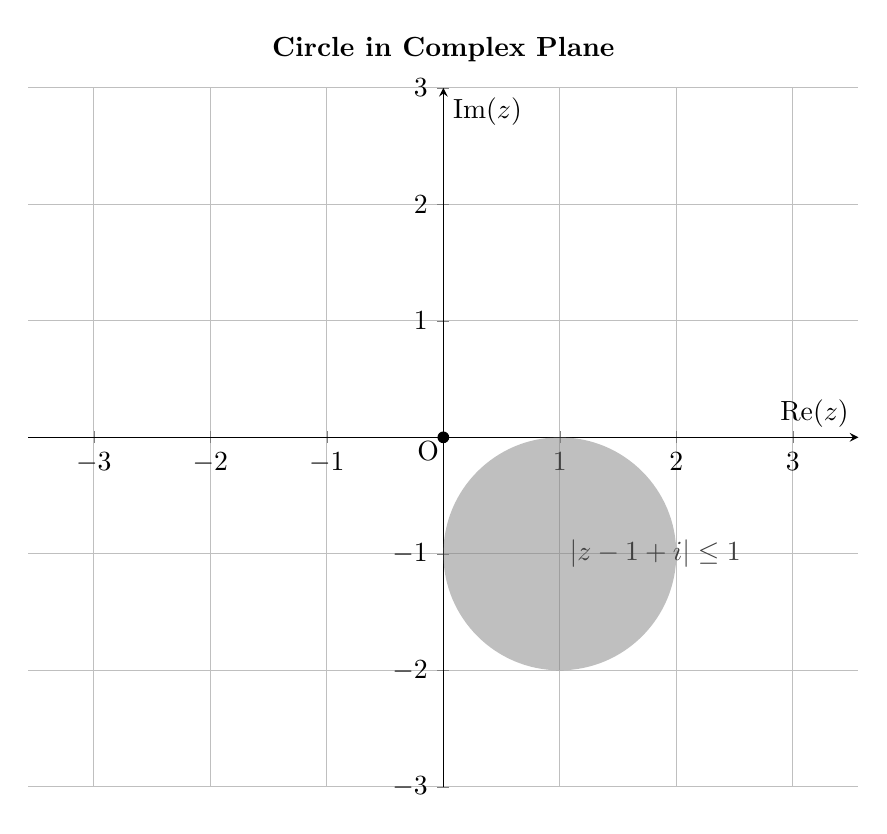
\begin{tikzpicture}
								\begin{axis}
									[
									title=\textbf{Circle in Complex Plane},
									xmin=-3,
									xmax=3,
									xtick distance={1},
									ymin=-3,
									ymax=3,
									ytick distance={1},
									axis lines=middle,
									grid,
									xlabel=Re$(z)$,
									ylabel=Im$(z)$,
									axis equal	
									]
									\node[label={[label distance=-5]225:{O}}, circle, fill, inner sep=1.5pt,] at (axis cs:0,0) {};
									
									\path [draw=none,fill=gray,semitransparent] (+1,-1) circle (1);
									\node [below,right,darkgray] at (+1,-1) {$|z-1+i| \leq 1$};
								\end{axis}
							\end{tikzpicture}
						\end{flushright}
					\end{minipage}
				\paragraph{Lines in the Complex Plane}\mbox{}\\
					\begin{minipage}{0.4\textwidth}
						Let $u,w\in\mathbb{C}$.\newline
						Therefore, $|z-u|=|z-w|$ defines the subset of $\mathbb{C}$ that are equidistant from $u$ and $w$. This is a straight line.
					\end{minipage}
					\hfill
					\begin{minipage}{0.6\textwidth}
						\begin{flushright}
							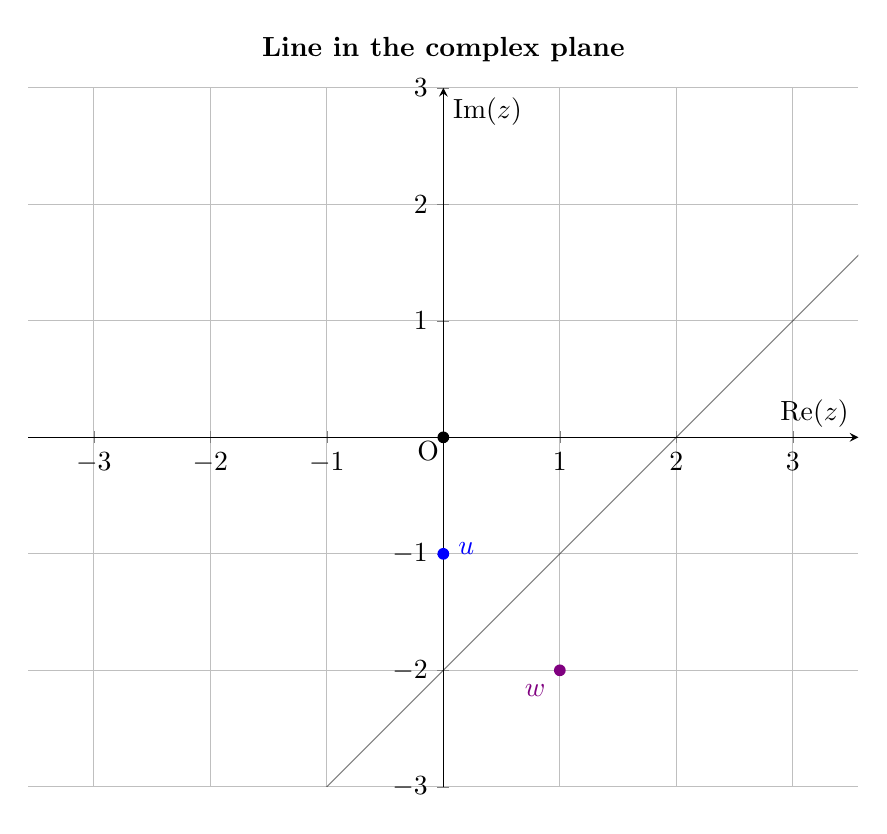
\begin{tikzpicture}
								\begin{axis}
									[
									title={\textbf{Line in the complex plane}},
									xmin=-3,
									xmax=3,
									xtick distance={1},
									ymin=-3,
									ymax=3,
									ytick distance={1},
									axis lines=middle,
									grid,
									xlabel=Re$(z)$,
									ylabel=Im$(z)$,
									axis equal	
									]
									
										\node[label={[label distance=-5]225:{O}}, circle, fill, inner sep=1.5pt,] at (axis cs:0,0) {};
										\draw [thin, semitransparent, >=stealth] (axis cs:-5,-7) [->](-5,-7) -- (8,6);
										\node[label={[right, text=blue, label distance=-5]225:{$u$}},circle,blue,fill,inner sep=1.5pt] at (axis cs:0,-1) {};
										\node[label={[text=violet, distance=-5]225:{$w$}},circle,violet,fill,inner sep=1.5pt] at (axis cs:1,-2){};
								\end{axis}
							\end{tikzpicture}
						\end{flushright}
					\end{minipage}
				\paragraph{Rays in the Complex Plane}\mbox{}\\
					\begin{minipage}[t]{0.5\textwidth}
						\vspace{0pt}
						\begin{flushleft}
							Let $\theta$ be a fixed angle. The equation $\Arg(z)=\theta$ defines a ray extending from the origin at an angle $\theta$ measured counterclockwise from the horizontal axis. $-\pi<\theta\leq\pi$.
						\end{flushleft}
					\end{minipage}
					\hfill
					\begin{minipage}[t]{0.5\textwidth}
						\vspace{0pt}
						\begin{flushright}
							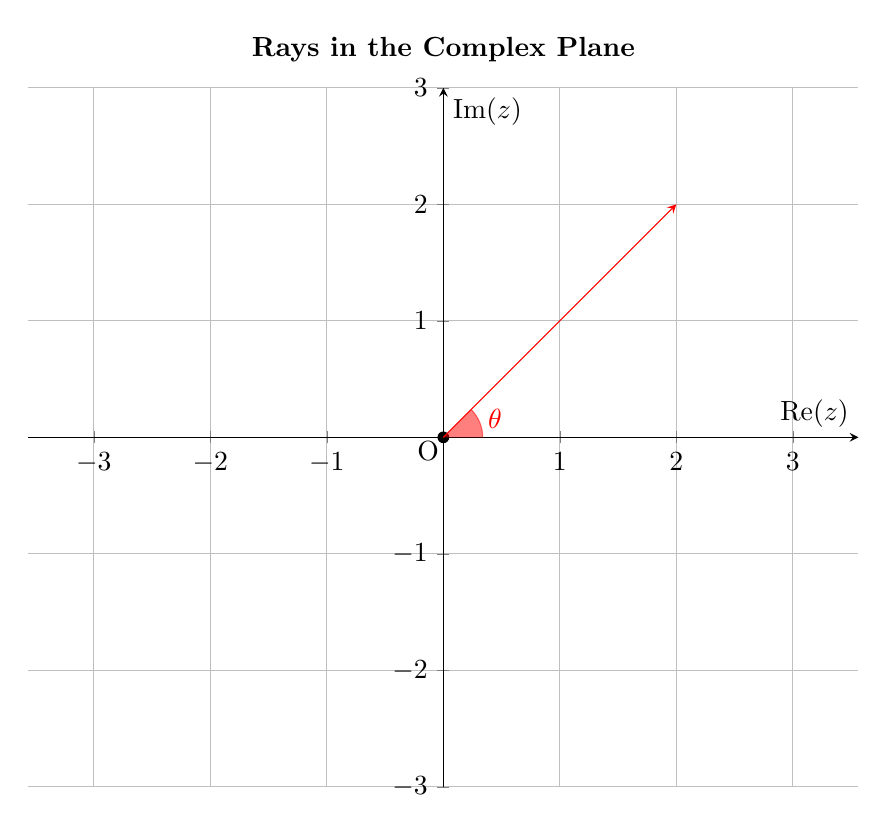
\begin{tikzpicture}
								\begin{axis}
									[
									title={\textbf{Rays in the Complex Plane}},
									xmin=-3,
									xmax=3,
									xtick distance={1},
									ymin=-3,
									ymax=3,
									ytick distance={1},
									axis lines=middle,
									grid,
									xlabel=Re$(z)$,
									ylabel=Im$(z)$,
									axis equal	
									]
									
									\node[label={[label distance=-5]225:{O}}, circle, fill, inner sep=1.5pt,] at (axis cs:0,0) {};
									
									\draw[thin, >=stealth, red] (axis cs:0,0) [->](0,0) -- (2,2);
									\begin{scope}
										\path[clip] (0,0) -- (2,0) -- (2,2);
										\fill[red, opacity=0.5, draw=red] (0,0) circle (5mm);
										\node[red] at ($(0,0)+(20:7mm)$) {$\theta$};
									\end{scope}
								\end{axis}
							\end{tikzpicture}
						\end{flushright}
					\end{minipage}\mbox{}\\
				\noindent\underline{Example}\newline
				Define sets $S$ and $T$ of complex numbers by:\newline
				$S=\{z: |z|\leq2\}$ and $T={z: Re(z)>1}$\newline
				Sketch $S\cap T$\newline
				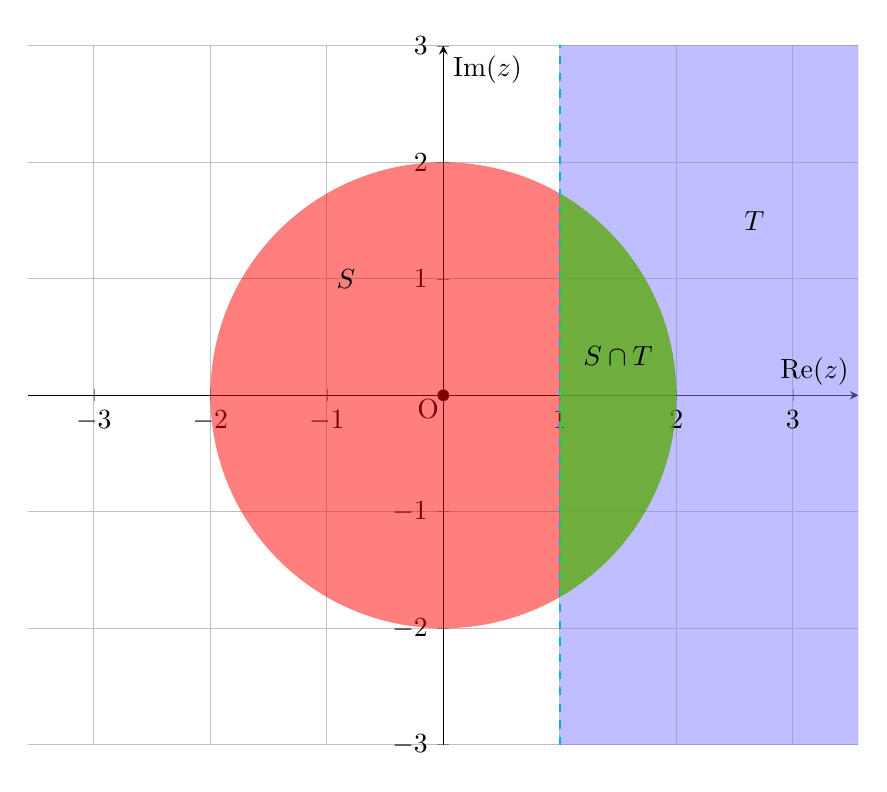
\begin{tikzpicture}
					\begin{axis}
						[
						xmin=-3,
						xmax=3,
						xtick distance={1},
						ymin=-3,
						ymax=3,
						ytick distance={1},
						axis lines=middle,
						grid,
						xlabel=Re$(z)$,
						ylabel=Im$(z)$,
						axis equal	
						]
						
						\node[label={[label distance=-5]225:{O}}, circle, fill, inner sep=1.5pt,] at (axis cs:0,0) {};
						
						\path [draw=none,fill=red,opacity=0.5] (+0,-0) circle (2);
						\node [below,right,black] at (-1,+1) {$S$};
						
						\addplot+[name path=A, cyan, dashed, thick] coordinates {(1,-5) (1,5)};
						\addplot+[name path=B, cyan, dashed, thick] coordinates {(5,-5) (5,5)};
						\addplot[name path=C, blue!50, opacity=0.5] fill between[of=A and B];
						\node [below,right,black] at (+2.5,+1.5) {$T$};
						
						\begin{scope}
							\clip (2,-5) rectangle (1,10);
							\fill[green, opacity=0.5](0,0) circle(2);
							\node [below,black] at (+1.5,+0.5) {$S\cap T$};
						\end{scope}
					\end{axis}
				\end{tikzpicture}
		\subsection{Vectors}
			\subsubsection{Introduction to Vectors}
				\paragraph{Directed Line Segments}\mbox{}\\
					A directed line segment from point A to point B is denoted by $\overrightarrow{AB}$ or $\utilde{a}$.
				\paragraph{Vectors in 2D}\mbox{}\\
					Let $\utilde{v}=x\utilde{i}+y\utilde{j}$ where $\utilde{i}$ and $\utilde{j}$ are unit vectors in the $x$ and $y$ directions respectively. \newline
					\newline
					Magnitude or length $= |\utilde{v}| = \sqrt{x^2+y^2}$\newline\newline
					Unit vector $=\hat{\utilde{v}}=\frac{1}{|\utilde{v}|}\cdot\utilde{v}$
				\paragraph{Position Vectors}\mbox{}\\
					Point $A(2,1)$ has the position vector $\overrightarrow{OA}=2\utilde{i}+\utilde{j}$ \newline
					Point $B(3,3)$ has the position vector $\overrightarrow{OB}=3\utilde{i}+3\utilde{j}$
			\subsubsection{Vector Operations}
				\paragraph{Vector Addition}\mbox{}\\
					\begin{minipage}{0.5\textwidth}
						\vspace{0pt}
						\begin{align*}
							\overrightarrow{OA}=\utilde{i}+\utilde{j}\text{ and }&\overrightarrow{OB}=-\utilde{i}+2\utilde{j} \\
							\therefore \overrightarrow{OA}+\overrightarrow{OB}&=(\utilde{i}+\utilde{j})+(-\utilde{i}+2\utilde{j}) \\
							&=3\utilde{j}
						\end{align*}
					\end{minipage}
					\begin{minipage}{0.5\textwidth}
						\vspace{0pt}
						\begin{flushright}
							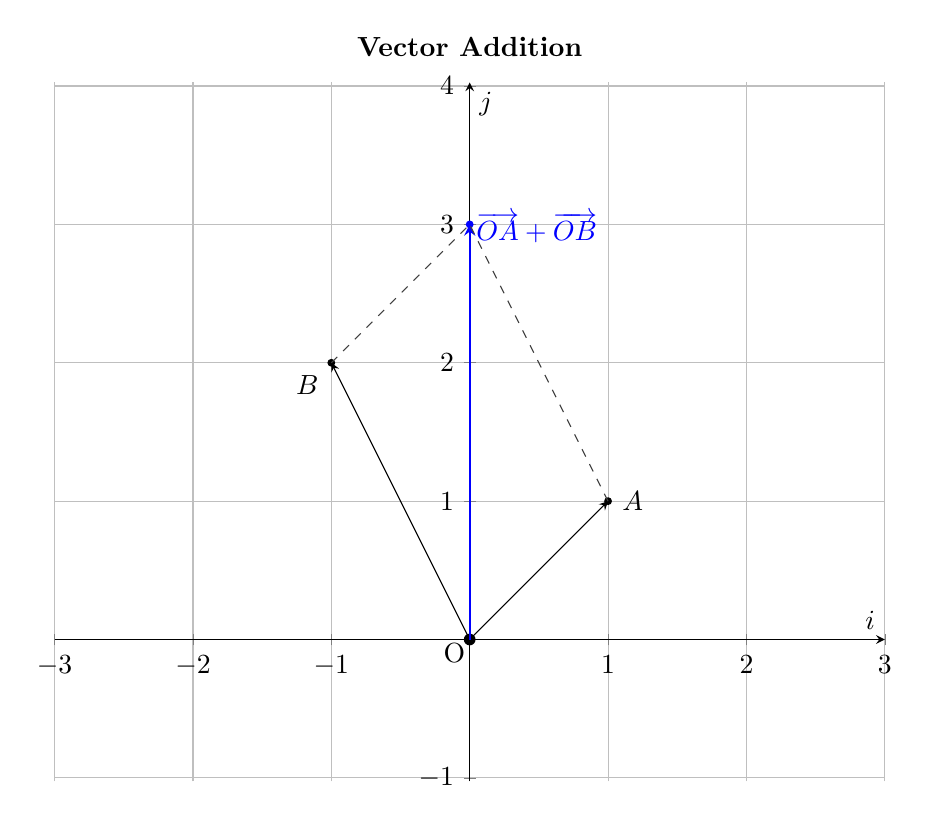
\begin{tikzpicture}
								\begin{axis}
									[
									title=\textbf{Vector Addition},
									xmin=-3,
									xmax=3,
									xtick distance={1},
									ymin=-1,
									ymax=4,
									ytick distance={1},
									axis lines=middle,
									grid,
									axis equal,
									xlabel=$\utilde{i}$,
									ylabel=$\utilde{j}$,
									]
									\node[label={[label distance=-5]225:{O}}, circle, fill, inner sep=1.5pt,] at (axis cs:0,0) {};
									
									\draw [thin,>=stealth] (axis cs:0,0) [->](0,0) -- (1,1);
									\node[label={0:{$A$}},circle, fill, inner sep=1pt] at (axis cs:1,1) {};
									
									\draw [thin, >=stealth] (axis cs:0,0) [->](0,0) -- (-1,2);
									\node[label={225:{$B$}},circle, fill, inner sep=1pt] at (axis cs:-1,2) {};
									
									\draw [thick, >=stealth, blue] (axis cs:0,0) [->](0,0) -- (0,3);
									\node[label={[text=blue,above,right]225:{$\overrightarrow{OA}+\overrightarrow{OB}$}},circle, fill, inner sep=1pt, blue] at (axis cs:0,3) {};
									
									\draw [dashed, thin, darkgray] (axis cs:1,2) (1,1) -- (0,3);
									\draw [dashed, thin, darkgray] (axis cs:-2,3) (-1,2) -- (0,3);
									
								\end{axis}
							\end{tikzpicture}
						\end{flushright}
					\end{minipage}
				\paragraph{Vector Subtraction}\mbox{}\\
					\begin{minipage}{0.5\textwidth}
						\vspace{0pt}
						$\overleftarrow{OB}-\overleftarrow{OA}=\overleftarrow{OB}+(-\overleftarrow{OA})$\newline
						To perform vector subtraction, we simply flip the vector that we are subtracting 180$^\circ$ and perform vector addition on these two new vectors.
					\end{minipage}
					\begin{minipage}{0.5\textwidth}
						\vspace{0pt}
						\begin{flushright}
							\begin{tikzpicture}
								\begin{axis}
									[
									title=\textbf{Vector Subtraction},
									xmin=-5,
									xmax=5,
									ymin=-7,
									ymax=3,
									axis lines=none,
									axis equal
									]
									
									\draw [thin, >=stealth] (axis cs:0,0) [->](0,0) -- (-2,3);
									\node [right,black] at (-1,+1.5) {$\utilde{a}$};
									
									\draw [thin, >=stealth] (axis cs:0,0) [->](0,0) -- (-4,-2);
									\node [below,black] at (-2,-1) {$\utilde{b}$};
									
									\draw [thin, red, >=stealth] (axis cs: 0,0) [->](0,0) -- (2,-3);
									\node [right,red] at (1,-1.5) {$-\utilde{a}$};
									
									\draw [dotted, thin, darkgray] (axis cs: 2,-3) (2,-3) -- (-2,-5);
									\draw [dotted, thin, darkgray] (axis cs: -4,-2) (-4,-2) -- (-2,-5);
									
									\draw [dashed, blue, >=stealth] (axis cs:0,0) [->](0,0) -- (-2,-5);
									\node [below,blue] at (-2,-5) {$\utilde{b}-\utilde{a}$};
									
								\end{axis}
							\end{tikzpicture}
						\end{flushright}
					\end{minipage}
				\paragraph{Scalar Multiplication}\mbox{}\\
					\begin{minipage}{0.5\textwidth}
						Multiplying a vector by a real number changes the length of the vector (magnitude).
					\end{minipage}
					\begin{minipage}{0.5\textwidth}
						\vspace{0pt}
						\begin{flushright}
							\begin{tikzpicture}
								\begin{axis}
									[
									title=\textbf{Scalar multiplication of Vectors},
									xmin=0,
									xmax=4,
									ymin=-1,
									ymax=5,
									axis lines=none,
									axis equal
									]
									
									\draw [thin, >=stealth] (axis cs:0,0) [->](0,0) -- (1,2);
									\node [right,black] at (-1,+1.5) {$\utilde{a}$};
									
									\draw [thin, >=stealth] (axis cs:1,0) [->](1,0) -- (3,4);
									\node [right,black] at (2,2) {$2\utilde{a}$};
									
								\end{axis}
							\end{tikzpicture}
						\end{flushright}
					\end{minipage}
			\subsubsection{Parallel, Position, and Zero Vectors}
				\paragraph{Zero Vector}\mbox{}\\
					The zero vector ($\utilde{0}$) has no magnitude and no direction.
				\paragraph{Parallel Vectors}\mbox{}\\
					Parallel vectors have the same or \textit{exact} opposite direction. \newline\newline
					\begin{Note}
						Two non-zero vectors are parallel if $\utilde{u}=k\utilde{v}$ where $k\in\mathbb{R}\setminus\{0\}$.
					\end{Note}
				\paragraph{Position Vectors}\mbox{}\\
					For any point $P(x,y)$ there is a position vector from the origin $\overrightarrow{OP}=\begin{bmatrix}
						x \\ y
					\end{bmatrix}$
			\subsubsection{Rectangular Components}
				\paragraph{Standard Unit Vectors}\mbox{}\\
					\begin{Note}
						A unit vector is a vector of length 1 unit in the same direction as a given vector.\\
						The unit vector of $\utilde{a}$ is denoted by $\hat{\utilde{a}}$.\\
						$|\utilde{a}|\times\hat{\utilde{a}}=\utilde{a}\;\;\;\;\therefore\hat{\utilde{a}}=\frac{1}{|\utilde{a}|}\times\utilde{a}$
					\end{Note}\mbox{}\\
					$\utilde{i}$ is the unit vector in the positive $x$ direction and $\utilde{j}$ is the unit vector in the positive $y$ direction.\newline
					\begin{minipage}{0.5\textwidth}
						$\utilde{u}=\overrightarrow{AB}=\begin{bmatrix}
							x \\ y
						\end{bmatrix}=x\utilde{i}+y\utilde{j}$\newline\newline
						$|\utilde{u}|=\sqrt{x^2+y^2}$
					\end{minipage}
					\begin{minipage}{0.5\textwidth}
						\begin{tikzpicture}
							\begin{axis}
								[
								title=\textbf{Vector Components},
								xmin=-3,
								xmax=3,
								xtick distance={1},
								xticklabel=\empty,
								yticklabel=\empty,
								ymin=-1,
								ymax=4,
								ytick distance={1},
								axis lines=middle,
								axis equal,
								xlabel=$\utilde{i}$,
								ylabel=$\utilde{j}$,
								]
								\node[label={[label distance=-5]225:{O}}, circle, fill, inner sep=1.5pt,] at (axis cs:0,0) {};
								
								\draw [thin,>=stealth] (axis cs:0,0) [->](1,1) -- (2,3);
								\node [left,black] at (1.5,2) {$\utilde{u}$};
								\node[below, left, black] at (1,1) {$A$};
								\node[above, right, black] at (2,3) {$B$};
								
								\draw [thick, dotted, blue] (axis cs:1,1) (1,1) -- (2,1);
								\draw [thick, dotted, blue] (axis cs:2,1) (2,1) -- (2,3);
								\node [below, blue] at (1.5,1) {$x$};
								\node [right, blue] at (2,2) {$y$};								
							\end{axis}
						\end{tikzpicture}
					\end{minipage}

			\subsubsection{Linear Combination of Non-Parallel Vectors}
				If two non-zero vectors $\utilde{a}$ and $\utilde{b}$ are not parallel and $m\utilde{a}+n\utilde{b}=p\utilde{a}+q\utilde{b}$ then $m=p$ and $n=q$.
			\subsubsection{Linear Dependence}
				A set of two vectors $\utilde{a}$ and $\utilde{b}$ are linearly dependent \textbf{if and only if} there exists $\lambda\in\mathbb{R}\setminus\{0\}$ such that $\utilde{a}=\lambda\utilde{b}$.
				\begin{align*}
					\utilde{a}&=2\utilde{i}-3\utilde{j}&\utilde{b}=4\utilde{i}-6\utilde{j} \\
					\utilde{b}&=2\utilde{a}&\therefore\text{ linear dependence}
				\end{align*}
				If no $\lambda\in\mathbb{R}\setminus\{0\}$ exists such that $\utilde{a}=\lambda\utilde{b}$, the vectors $\utilde{a}$ and $\utilde{b}$ are said to be linearly independent.
				\paragraph{Linear Dependence of 3 Vectors}\mbox{}\\
					Let $\utilde{a},\utilde{b}$ be non-zero vectors that are not parallel. $\utilde{a},\utilde{b},\utilde{c}$ are linearly dependent \textbf{if and only if} there exists $m,n\in\mathbb{R}$ such that $\utilde{c}=m\utilde{a}+n\utilde{b}$
			\subsubsection{Scalar Product}
				If $\utilde{a}=a_1\utilde{i}+a_2\utilde{j}$ and $\utilde{b}=b_1\utilde{i}+b_2\utilde{j}$, then $\utilde{a}\cdot\utilde{b}=a_1b_1+a_2b_2$
				\paragraph{Geometric Description of Dot Product}\mbox{}\\
				\[
					\utilde{a}\cdot\utilde{b}=|\utilde{a}|\times|\utilde{b}|\times\cos\theta
				\]
				\begin{minipage}{0.5\textwidth}
					$\theta$ is defined as the angle where both 'hats' of the vectors are.
				\end{minipage}
				\hfill
				\begin{minipage}{0.5\textwidth}
					\begin{flushright}
						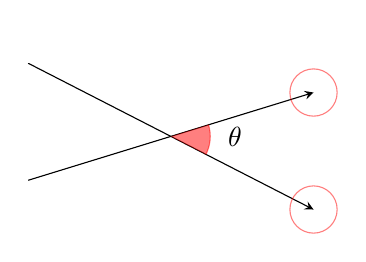
\begin{tikzpicture}
							\begin{axis}
								[
								title=\empty,
								xmin=-5,
								xmax=5,
								xtick distance={1},
								xticklabel=\empty,
								yticklabel=\empty,
								ymin=-7,
								ymax=5,
								ytick distance={1},
								axis lines=none,
								xlabel=$\utilde{i}$,
								ylabel=$\utilde{j}$,
								width=3in,
								height=1.5in
								]
								\draw [thin,>=stealth] (axis cs:0,0) [->](-3,-3) -- (3,3);
								\draw [thin, >=stealth] (axis cs:0,0) [->](-3,5) -- (3,-5);
								
								\begin{scope}
									\path[clip] (0,0) -- (3,3) -- (3,-5);
									\fill[red, opacity=0.5, draw=red] (0,0) circle (5mm);
									\node [right] at (axis cs:1,0) {$\theta$};
								\end{scope}
								\path [draw=none, draw=red, semitransparent] (3,3) circle (3mm);
								\path [draw=none, draw=red, semitransparent] (3,-5) circle (3mm);
							\end{axis}
						\end{tikzpicture}
					\end{flushright}
				\end{minipage}
				When $\utilde{a}\cdot\utilde{b}=0$, the vectors are perpendicular (incident at 90$^\circ$ angle) as $cos(90^\circ)=0$
				\paragraph{Simplifying Expressions of Dot Products}\mbox{}\\
					\underline{Example}\newline
					Expand and simplify:\newline
					\begin{minipage}{0.5\textwidth}
						(a) $\utilde{a}\cdot(\utilde{a}+\utilde{b})-\utilde{a}\cdot\utilde{b}$\newline
						\[
						=\utilde{a}^2+\utilde{a}\cdot\utilde{b}-\utilde{a}\cdot\utilde{b}=\utilde{a}^2=|\utilde{a}|^2
						\]
					\end{minipage}
					\hfill
					\begin{minipage}{0.5\textwidth}
						(b) $(\utilde{a}\cdot\utilde{b})\cdot(\utilde{a}-\utilde{b})$\newline
						\[
						=\utilde{a}^2-\utilde{a}\cdot\utilde{b}+\utilde{b}\cdot\utilde{a}-\utilde{b}^2=\utilde{a}^2-\utilde{b}^2=|\utilde{a}|^2-|\utilde{b}|^2
						\]
					\end{minipage}
			\subsubsection{Scalar and Vector Projections/Resolute}
				\begin{minipage}[t]{0.5\textwidth}
					\vspace{0pt}
					\begin{flushleft}
						\begin{tikzpicture}
							\begin{axis}
								[
								title=\empty,
								xmin=-1,
								xmax=6,
								xtick distance={1},
								xticklabel=\empty,
								yticklabel=\empty,
								ymin=-2,
								ymax=5,
								ytick distance={1},
								axis lines=none,
								xlabel=$\utilde{i}$,
								ylabel=$\utilde{j}$,
								width=3in,
								height=1.5in
								]
								\draw [thin,>=stealth] (axis cs:0,0) [->](0,0) -- (3,4);
								\node [above, left] at (axis cs: 1.5,2){$\utilde{a}$};
								\draw [thin, >=stealth] (axis cs:0,0) [->](0,0) -- (5,0);
								\node [below] at (axis cs: 2.5,0){$\utilde{b}$};
								
								\draw[thick, magenta, dashed] (axis cs:0,0) (0,0) -- (3,0);
								\node[above, magenta] at (axis cs:2,0){$\utilde{u}$};
								
								\draw[thick, magenta, dashed] (axis cs:3,0) (3,0) -- (3,4);
								\node[right, magenta] at (axis cs:3,2){$\utilde{w}$};
							\end{axis}
						\end{tikzpicture}
					\end{flushleft}
				\end{minipage}
				\begin{minipage}[t]{0.5\textwidth}
					\vspace{0pt}
					It is often useful to decompose vector $\utilde{a}$ into the sum of two vectors, where one is perpendicular to $\utilde{b}$ and the other parallel to $\utilde{b}$.\newline\newline
					In the example left, $\utilde{u}$ is parallel to $\utilde{b}$ and $\utilde{w}$ is perpendicular to $\utilde{b}$.
				\end{minipage}
				\[
					\utilde{a}=\utilde{u}+\utilde{w}\text{ where }\utilde{w}\perp\utilde{b},\;\;\utilde{u}\parallel\utilde{b}
				\]
				\begin{align*}
					\utilde{u}&=k\utilde{b}\text{ as }\utilde{u}\parallel\utilde{b}\therefore k\in\mathbb{R} \\
					\utilde{w}&=\utilde{a}-\utilde{u} \\
					&=\utilde{a}-k\utilde{b} \\\\
					(\utilde{a}-k\utilde{b})\cdot\utilde{b}&=0\text{ as }\utilde{w}\perp\utilde{b} \\
					\utilde{a}\utilde{b}-k\utilde{b}^2&=0 \\
					\utilde{a}\cdot\utilde{b}&=k\utilde{b}^2 \\
					k&=\frac{\utilde{a}\cdot\utilde{b}}{|\utilde{b}|^2} \\\\
					\therefore\utilde{u}&=k\utilde{b} \\
					&=\frac{\utilde{a}\cdot\utilde{b}}{|\utilde{b}|^2}\cdot\utilde{b}
				\end{align*}
				\paragraph{Vector Resolute (Vector Projection)}\mbox{}\\
				The vector resolute of $\utilde{a}$ in direction $\utilde{b}$ is given by:
				\[
					\utilde{u}=\frac{\utilde{a}\cdot\utilde{b}}{|\utilde{b}|^2}\cdot\utilde{b}\;\;\;\text{ OR }\;\;\;\utilde{u}=\utilde{a}\cdot\hat{\utilde{b}}\cdot\utilde{b}
				\]
				\paragraph{Scalar Resolute}\mbox{}\\
				The scalar resolute does not include the direction of the resolution. It is given by:
				\[
					\utilde{a}\cdot\hat{\utilde{b}}=\frac{\utilde{a}\cdot\utilde{b}}{|\utilde{b}|}
				\]
				\underline{Example}\newline
				Let $\utilde{a}=\utilde{i}+3\utilde{j},\;\utilde{b}=\utilde{i}-\utilde{j}$.\newline
				(a) Find the scalar resolute of $\utilde{a}$ in direction $\utilde{b}$\newline
				\[
					\utilde{a}\cdot\hat{\utilde{b}}=\frac{\utilde{a}\cdot\utilde{b}}{|\utilde{b}|}=\frac{1(1)+3(-1)}{\sqrt{1^2+(-1)^2}}=\frac{-2}{\sqrt{2}}=-\sqrt{2}
				\]
				(b) Find the vector resolute of $\utilde{a}$ in direction $\utilde{b}$\newline
				\begin{minipage}[t]{0.5\textwidth}
					\begin{align*}
						\utilde{u}&=\frac{\utilde{a}\cdot\utilde{b}}{|\utilde{b}|^2}\cdot\utilde{b} \\
						&=\frac{1(1)+3(-1)}{(\sqrt{1^2+(-1)^2})^2}\cdot\utilde{b} \\
						&=\frac{-2}{2}\cdot\utilde{b}=-1(\utilde{i}-\utilde{j}) \\
						\utilde{u}&=-\utilde{i}+\utilde{j}
					\end{align*}
				\end{minipage}
				\hfill
				\begin{minipage}[t]{0.5\textwidth}
					\begin{align*}
						\utilde{a}&=\utilde{u}+\utilde{w} \\
						\therefore\utilde{w}&=\utilde{a}-\utilde{u} \\
						&=\utilde{i}+3\utilde{j}-(-\utilde{i}+\utilde{j}) \\
						&=2\utilde{i}+2\utilde{j}
					\end{align*}
				\end{minipage}
				(c) Find the vector resolute of $\utilde{b}$ in direction $\utilde{a}$\newline
				\begin{minipage}[t]{0.5\textwidth}
					\begin{align*}
						\utilde{u}&=\frac{\utilde{b}\cdot\utilde{a}}{|\utilde{a}|^2}\cdot\utilde{a} \\
						&=\frac{3(-1)+1(1)}{(\sqrt{10})^2}\cdot\utilde{a} \\
						&=-\frac{1}{5}\utilde{a} \\
						&=-\frac{1}{5}\utilde{i}-\frac{3}{5}\utilde{j}
					\end{align*}
				\end{minipage}
				\hfill
				\begin{minipage}[t]{0.5\textwidth}
					\begin{align*}
						\utilde{b}&=\utilde{u}+\utilde{w} \\
						\therefore\utilde{w}&=\utilde{b}-\utilde{u} \\
						&=\utilde{i}-\utilde{j}-(-\frac{1}{5}\utilde{i}-\frac{3}{5}\utilde{j}) \\
						w&=\frac{6}{5}\utilde{i}-\frac{2}{5}\utilde{j}
					\end{align*}
				\end{minipage}
				
			\subsubsection{Co-linearity}
				\begin{minipage}{0.5\textwidth}
					3 points are co-linear if $\overrightarrow{AB}=k\overrightarrow{AC}$ or $\overleftarrow{AB}=k\overleftarrow{BC}$.\newline\newline
					\begin{Note}
						In order to be co-linear, the two vectors being compared must have a common point.
					\end{Note}
				\end{minipage}
				\hfill
				\begin{minipage}{0.5\textwidth}
					\begin{flushright}
						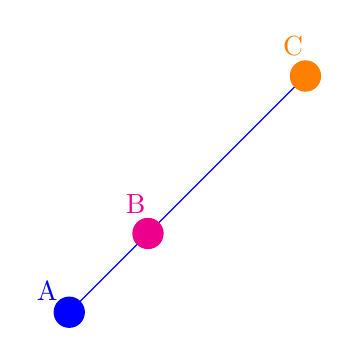
\begin{tikzpicture}
							\draw[blue] (0,0) -- (3,3);
							\node[label={[text=blue, label distance=-5]500:{A}}, circle, fill, blue, inner sep=4pt,] at (0,0) {};
							\node[label={[text=magenta, left, above]500:{B}}, circle, fill, magenta, inner sep=4pt] at (1,1) {};
							\node[label={[text=orange, above]500:{C}}, circle, fill, orange, inner sep=4pt] at (3,3){};
						\end{tikzpicture}
					\end{flushright}
				\end{minipage}
			\subsubsection{Vector Proofs}
				\begin{enumerate}
					\item Draw a diagram
					\item Write down what you know
					\item Write down what to show
					\item LHS and RHS of show and make them equal
				\end{enumerate}
				\underline{Example}\newline
				Using your knowledge of vectors, prove the cosine rule.\newline
				\begin{minipage}{0.5\textwidth}
					\textbf{Know:} $\utilde{c}=\utilde{b}-\utilde{a}$\newline
					\textbf{Show:} $|\utilde{c}|^2=|\utilde{a}|^2+|\utilde{b}|^2-2|\utilde{a}||\utilde{b}|\cos\theta$\newline
				\end{minipage}
				\hfill
				\begin{minipage}{0.5\textwidth}
					\begin{flushright}
						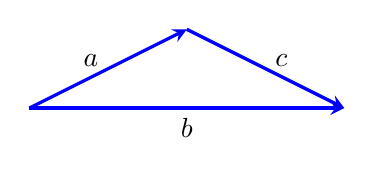
\begin{tikzpicture}
							\draw[very thick, blue, >=stealth] [->](0,0) -- (4,0);
							\node[below] at (2,0){$\boldmath{\utilde{b}}$};
							\draw[very thick, blue, >=stealth] [->](0,0) -- (2,1);
							\node[above=0.1, left] at (1,0.5){$\boldmath{\utilde{a}}$};
							\draw[very thick, blue, >=stealth] [->](2,1) -- (4,0);
							\node[above=0.1, right] at (3,0.5){$\boldmath{\utilde{c}}$};
						\end{tikzpicture}
					\end{flushright}
				\end{minipage}
				\begin{align*}
					\text{LHS}&=|\utilde{c}|^2 \\
					&=\utilde{c}\cdot\utilde{c} \\
					&=(\utilde{b}-\utilde{a})\cdot(\utilde{b}-\utilde{a})\;\text{ as }\utilde{c}=\utilde{b}-\utilde{a} \\
					&=\utilde{b}\cdot\utilde{b}-\utilde{a}\cdot\utilde{b}-\utilde{a}\cdot\utilde{b}+\utilde{a}\cdot\utilde{a} \\
					&=|\utilde{a}|^2+|\utilde{b}|^2-2\utilde{a}\cdot\utilde{b} \\
					&=|\utilde{a}|^2+|\utilde{b}|^2-2|\utilde{a}||\utilde{b}|\cos\theta \\
					\text{LHS}&=\text{RHS}\qed
				\end{align*}
			\subsubsection{Vector Functions and Vector Kinematics}
				\paragraph{Vector Function}\mbox{}\\
					Consider the vector function $\utilde{r}(t)=t\utilde{i}+(t+2)\utilde{j}$ \newline
					$\utilde{r}(t)$ represents a family of vectors defined by different values of $t$.
				\paragraph{Finding Cartesian Equation}\mbox{}\\
					\begin{align*}
						\utilde{r}(t)&=x\utilde{i}+y\utilde{j} \\
						\utilde{r}(t)&=t\utilde{i}+(t+2)\utilde{j} \\
						x=t&\text{ and }y=t+2\;\therefore\;y=x+2
					\end{align*}
					\newpage
					\noindent\underline{Example}\newline
					The position vector $\utilde{r}(t)$ of a particle moving relative to the origin at time $t$ seconds is given by:
					\[
						\utilde{r}(t)=2\cos(t)\utilde{i}-3\sin(t)\utilde{j}
					\]
					Find the cartesian equation and state the domain and range.\newline
					\begin{minipage}[t]{0.5\textwidth}
						\vspace{0pt}
						\begin{align*}
							x=2\cos(t)&\implies\cos(t)=\frac{x}{2} \\
							y=-3\sin(t)&\implies\sin(t)=-\frac{y}{3} \\\\
							\sin^2(t)&+\cos^2(t)=1 \\
							\left(\frac{x}{2}\right)^2&+\left(-\frac{y}{3}\right)^2=1 \\\\
							\frac{x^2}{4}&+\frac{y^2}{9}=1\text{ (Ellipse)}
						\end{align*}
					\end{minipage}
					\hfill
					\begin{minipage}[t]{0.5\textwidth}
						\vspace{0pt}
						\begin{align*}
							&\textbf{Domain}\\
							&x=2\cos(t)\rightarrow 2\cos(t)\in\left[-2,2\right] \\
							&\therefore x_{cartesian}\in\left[-2,2\right] \\\\
							&\textbf{Range} \\
							&y=-3\sin(t)\rightarrow -3\sin(t)\in\left[-3,3\right] \\
							&\therefore y_{cartesian}\in\left[-3,3\right] \\
						\end{align*}
					\end{minipage}
				\paragraph{Position, Velocity, Acceleration as Vector Functions}\mbox{}\\
				We can describe position, velocity, and acceleration as vector functions. The general forms of these functions are written below.
				\bgroup
				\def\arraystretch{2.5}
				\begin{table}[H]
					\centering
					\begin{tabular}{|l|l|}
						\hline
						Position Vector & $\utilde{r}(t)=x(t)\utilde{i}+y(t)\utilde{j}$ \\
						\hline
						Velocity Vector & $\utilde{v}(t)=\dot{x}(t)\utilde{i}+\dot{y}(t)\utilde{j}$ \\
						\hline
						Acceleration Vector & $a(t)=\dot{\utilde{v}}(t)=\ddot{\utilde{r}}=\ddot{x}(t)\utilde{i}+\ddot{y}(t)\utilde{j}$\\
						\hline
						Distance from O & $|\utilde{r}(t)|=\sqrt{(x(t))^2+(y(t))^2}$ \\
						\hline
						Speed & $|\utilde{v}(t)|=\sqrt{(\dot{x}(t))^2+(\dot{y}(t))^2}$ \\
						\hline
						Magnitude of Acceleration & $|\utilde{a}(t)|=\sqrt{(\ddot{x}(t))^2+(\ddot{y}(t))^2}$ \\
						\hline
					\end{tabular}
				\end{table}
				\egroup
				\begin{Note}
					$\dot{f}(t)$ denotes the first derivative of function $f$. \\
					$\ddot{f}(t)$ denotes the second derivative of function $f$.
				\end{Note}
\end{document}